%%%%%%%%%%%%%%%%%%%%%%%%%%%%%%%%%%%%%%%%%%%%%%%%%%%%%%%%%%%%
%%% LIVECOMS ARTICLE TEMPLATE FOR BEST PRACTICES GUIDE
%%% ADAPTED FROM ELIFE ARTICLE TEMPLATE (8/10/2017)
%%%%%%%%%%%%%%%%%%%%%%%%%%%%%%%%%%%%%%%%%%%%%%%%%%%%%%%%%%%%
%%% PREAMBLE
\documentclass[9pt,tutorial]{livecoms}
% Use the 'onehalfspacing' option for 1.5 line spacing
% Use the 'doublespacing' option for 2.0 line spacing
% Use the 'lineno' option for adding line numbers.
% Use the "ASAPversion' option following article acceptance to add the DOI and relevant dates to the document foothttps://www.overleaf.com/project/5f085f02498a0400013493c4er.
% Use the 'pubversion' option for adding the citation and publication information to the document footer, when the LiveCoMS issue is finalized.
% The 'bestpractices' option for indicates that this is a best practices guide.
% Omit the bestpractices option to remove the marking as a LiveCoMS paper.
% Please note that these options may affect formatting.

\usepackage{lipsum} % Required to insert dummy text
\usepackage[version=4]{mhchem}
\usepackage{siunitx}
\DeclareSIUnit\Molar{M}
\usepackage[italic]{mathastext}
\graphicspath{{figures/}}
\usepackage{listings}
\lstset{basicstyle=\ttfamily,breaklines=true}
\usepackage{hyperref}
\usepackage{textcomp}
%%%%%%%%%%%%%%%%%%%%%%%%%%%%%%%%%%%%%%%%%%%%%%%%%%%%%%%%%%%%
%%% IMPORTANT USER CONFIGURATION
%%%%%%%%%%%%%%%%%%%%%%%%%%%%%%%%%%%%%%%%%%%%%%%%%%%%%%%%%%%%

\newcommand{\versionnumber}{1.0}  % you should update the minor version number in preprints and major version number of submissions.
\newcommand{\githubrepository}{\url{https://github.com/TUNNELING-GROUP/aqua-duct_tutorials_livecoms}}  %this should be the main github repository for this article

%%%%%%%%%%%%%%%%%%%%%%%%%%%%%%%%%%%%%%%%%%%%%%%%%%%%%%%%%%%%
%%% ARTICLE SETUP
%%%%%%%%%%%%%%%%%%%%%%%%%%%%%%%%%%%%%%%%%%%%%%%%%%%%%%%%%%%%
\title{AQUA-DUCT: Analysis of Molecular Dynamics Simulations of Macromolecules with the Use of Molecular Probes [Article v\versionnumber]}

\author[1\authfn{1}]{Karolina Mitusińska}
\author[1\authfn{1}]{Agata Raczyńska}
\author[1\authfn{1}]{Piotr Wojsa}
\author[1,2\authfn{1}]{Maria Bzówka}
\author[1*]{Artur Góra}
\affil[1]{Tunneling Group, Biotechnology Centre, Silesian University of Technology, Bolesława Krzywoustego 8, Gliwice, Poland}
\affil[2]{Department of Organic Chemistry, Bioorganic Chemistry and Biotechnology, Faculty of Chemistry, Silesian University of Technology, Bolesława Krzywoustego 4, Gliwice, Poland}

\corr{a.gora@tunnelinggroup.pl}{AG}

\orcid{Karolina Mitusińska}{0000-0002-0183-0845}
\orcid{Agata Raczyńska}{0000-0002-1884-3669}
\orcid{Piotr Wojsa}{0000-0002-1013-7137}
\orcid{Maria Bzówka}{0000-0001-6802-8753}
\orcid{Artur Góra}{0000-0003-2530-6957}

\contrib[\authfn{1}]{These authors contributed equally to this work}
%\contrib[\authfn{2}]{These authors also contributed equally to this work}

%\presentadd[\authfn{3}]{Department, Institute, Country}
%\presentadd[\authfn{4}]{Department, Institute, Country}

\blurb{This LiveCoMS document is maintained online on GitHub at \githubrepository; to provide feedback, suggestions, or help improve it, please visit the GitHub repository and participate via the issue tracker.}

%%%%%%%%%%%%%%%%%%%%%%%%%%%%%%%%%%%%%%%%%%%%%%%%%%%%%%%%%%%%
%%% PUBLICATION INFORMATION
%%% Fill out these parameters when available
%%% These are used when the "pubversion" option is invoked
%%%%%%%%%%%%%%%%%%%%%%%%%%%%%%%%%%%%%%%%%%%%%%%%%%%%%%%%%%%%
\pubDOI{10.XXXX/YYYYYYY}
\pubvolume{<volume>}
\pubissue{<issue>}
\pubyear{<year>}
\articlenum{<number>}
\datereceived{Day Month Year}
\dateaccepted{Day Month Year}

%%%%%%%%%%%%%%%%%%%%%%%%%%%%%%%%%%%%%%%%%%%%%%%%%%%%%%%%%%%%
%%% ARTICLE START
%%%%%%%%%%%%%%%%%%%%%%%%%%%%%%%%%%%%%%%%%%%%%%%%%%%%%%%%%%%%

\begin{document}
\lstset{upquote=true}
\begin{frontmatter}
\maketitle

\begin{abstract}
% limit: 250 words, currently: 135 words
AQUA-DUCT software reverses the standard approach of the molecular dynamics simulations analysis of macromolecules, focusing on solvent, co-solvent and small ligands analysis considered as specific molecular probes instead of analysis of macromolecules atoms movement. Here we present six basic tutorials instructing the users in the best practices for preparing, carrying out, and analysing AQUA-DUCT results in various applications. Users are expected to already have significant experience with running standard molecular dynamics simulations in any dedicated software (e.g., Amber, GROMACS, NAMD), and usage of PyMOL visualising software. The tutorials range from a basic analysis of multiple solvents trajectory used for identification of the entries/exits to the protein core, to a complex one, like identification of the key hot-spots in co-solvent MD simulations that can be used as an insight for macromolecules description, analysis, re-engineering, and for drug design. 

\end{abstract}

\end{frontmatter}

\section{Introduction}

One of the most extensively used methods for the \textit{in silico} study of macromolecules is  molecular dynamics (MD) simulation. The power of state-of-the-art MD simulations has been used for validating and extending results provided by NMR, terahertz (THz) absorption spectroscopy, and other experimental techniques \cite{Bottaro2018}. The accuracy of MD simulations’ predictions has increased due to:  i) continuous improvements in the force fields describing the interatomic interactions of folded and intrinsically disordered proteins \cite{Huang2017}; and ii) the ability to capture events taking place over longer periods of time using enhanced sampling methods \cite{Bernardi2015} and Markov models \cite{Husic2018}. MD simulations have increased our knowledge of the conformational changes of proteins’ regulatory elements such as gates \cite{Gora2013} or loops \cite{Kress2018}. It improved our understanding of the role of water in protein folding and stability, in shaping enzyme’s activity and selectivity, or in drug design \cite{Mondal2017,Spyrakis2017}. Finally, MD simulations enabled analysis of intramolecular voids, described as cavities \cite{Stank2016} and tunnels \cite{Kingsley2015,Marques2016}, which contribute to the macromolecules’ stability, functionality, activity, and selectivity \cite{Kokkonen2019}. More than 64\% of enzymes are equipped with active sites buried inside the protein core \cite{Pravda2014}, and investigation of the ligands’ entry pathways is considered as essential for future improvements in \textit{de novo} designed enzymes \cite{Huang2016}. However, the description of protein interior dynamics is not a trivial problem. The commonly used sphere approximation fails to give an accurate description of asymmetric volumes and neglects the physico-chemical properties of the interior – factors essential for analysis of the transportation of ligands or reagents \cite{Kaushik2018}.

AQUA-DUCT is an open-source Python software, designed for the analysis of macromolecules from the intramolecular voids perspective using small ligands as molecular probes. Key features of AQUA-DUCT include: i) identification of the functionally relevant tunnels, ii) statistical analysis of the solvent flow through tunnel network, iii) identification of structurally important residues and/or regions of macromolecules, iv) approximation of free energy profiles of transportation pathways, and v) an analysis of the evolution of the voids’ and hot-spots dynamics, based on the results of any molecular dynamics simulations. The software includes also script for results manipulation in PyMOL \cite{Delano2002} software as well as own graphical user interface (GUI) and a module for statistical data presentation. 

AQUA-DUCT is:
\newline
i) system independent - it enables the analysis of MD simulations generated by the most popular MD simulation software (i.e., AMBER, NAMD, GROMACS, and more), 
\newline
ii) ligands independent - it can trace flow of water, co-solvents, small ligands, or ions, also within one calculation, 
\newline
iii) highly flexible - the user can adjust the areas of interests (i.e., the \emph{Scope} and \emph{Object}), determine which tunnels entrances to inspect, analyse single or multiple simulations, analyse whole simulations or only some interesting parts to examine the time evolution of the system. 

Moreover, AQUA-DUCT enables time dependent/independent analysis which means that the user can use one software to get both the global statistic of your system as well as time dependent analysis (e.g., information about your system in different conformational states) together with the information about the time evolution of the system. As for our knowledge, AQUA-DUCT is one of the few software that can provide access to information vital for protein engineering and drug design during single analysis. The applicability of AQUA-DUCT software covers detailed analysis of small molecules transportation through protein, facilitation of protein re-engineering and drug design. 

\subsection{Scope}

This article presents six tutorials which explain all available functionalities in AQUA-DUCT \cite{Magdziarz2020}. They are as follows:
\begin{enumerate}
\item Basic solvent transportation analysis
\item Advanced solvent transportation analysis: multi-level clustering and visualization tips
\item Quantitative analysis and visualization of the results
\item Local distribution approach: hot-spots identification and energy profiles
\item Time-window analysis
\item Multiple solvent analysis
\end{enumerate}

The first Tutorial explains how to perform basic analysis with AQUA-DUCT and each of the following ones explain how the analysis can be extended to gain more information about the investigated system. If the user is already familiar with some of the AQUA-DUCT functions, they can move to the particular section that interests them. 

Tutorial 1, “Basic solvent transportation analysis”, comprises the essential options for running AQUA-DUCT calculations. It explains basic AQUA-DUCT functions and terms. The user will learn how to use the main module of AQUA-DUCT, \textit{valve}, through using the Graphical User Interface (GUI), Valve Configurator, and prepare the input files. After completing this tutorial, the user should be able to run basic AQUA-DUCT calculations. The objectives of this tutorial are to perform an analysis of the small molecules flow through the enzyme's interior, and to compare the identified tunnels. Specific learning objectives include:
\begin{enumerate}
  \item Understand and apply the definition of Scope and Object
  \item Carry out steps of configuration file preparation using GUI Valve Configurator
  \item Comprehend function of specific options in individual steps of calculations and how to set them
  \item Run basic calculations
  \item Visualize the results.
\end{enumerate}

Tutorial 2, “Advanced solvent transportation analysis: multi-level clustering and visualization tips”, represents a continuation and extension of the previous Tutorial 1 “Basic solvent transportation analysis”. It extends information about available options in AQUA-DUCT and explains how to improve results from Tutorial 1 by using advanced inlets clustering options and how to enhance visualization of the results. The objectives of this tutorial are to identify the entrances/exits to the enzyme's active site, and analyse the directions of the solvent flow. After completing this tutorial, the user should be able to:
\begin{enumerate}
  \item Perform advanced clustering, even in a case where several iterations of clustering should be performed
  \item Join divided clusters and create a cluster of outliers
  \item Repeat calculations from a chosen stage rather than again from the beginning
  \item Understand what visualized results represent
  \item Perform advanced analysis of the visualized results.
\end{enumerate}

Tutorial 3, “Quantitative analysis and visualization of the results”, explains how to use \textit{kraken}, which is a small and smart GUI application that helps to gather all quantitative results from AQUA-DUCT, therefore facilitating the analysis of the text result files. The objective of this tutorial is to analyse the available statistical data obtained during the solvent flow analysis. After completing this tutorial, the user should be able to:
\begin{enumerate}
  \item Provide files needed to run \textit{kraken}
  \item Understand what numerous plots from \textit{kraken} results indicate.
\end{enumerate}

Tutorial 4, “Advanced solvent transportation analysis: hot-spots identification and energy profiles”, presents another AQUA-DUCT module - \textit{pond}, that performs hot-spots and energy profiles calculations. The objectives of this tutorial are to understand the local solvent distribution approach, identify the most "attractive" regions within the enzyme's interior, and calculate an energy profile along a selected path, using a combination of the local solvent approach and the solvent transportation analysis. After completing this tutorial, the user should be able to:
\begin{enumerate}
  \item Carry out configuration file preparation using \textit{valve} template configuration file
  \item Run \textit{pond} module
  \item Visualize and understand hot-spots and pockets results
  \item Resize hot-spots
  \item Calculate energy profile and visualize it.
\end{enumerate}

Tutorial 5, ”Time-window analysis”, shows how to run calculations in fixed time-windows rather than analyse the whole system evolution at once. The objectives of this tutorial are to use the time-window analysis to identify hot-spots, and calculate an energy profile along a selected path, with respect to the time evolution of the analysed system. After completing this tutorial, the user should be able to:
\begin{enumerate}
  \item Run time-window analysis
  \item Analyse the trajectory in pre-defined time windows 
  \item Identify equivalent or alternative states. 
\end{enumerate}

Tutorial 6, "Multiple solvents analysis" explains how to analyse system with more than one solvent in order to calculate hot-spots and pockets of different solvents using AQUA-DUCT module - \textit{pond}. The objective of this tutorial is to run a hot-spots analysis using different solvent molecules with different physico-chemical properties. After completing this tutorial, the user should be able to:
\begin{enumerate}
  \item Run calculations considering the presence of more than one solvent in the system
  \item Run \textit{pond} module on a system with multiple solvents
  \item Visualize, resize and analyse hot-spots from multiple solvents.
\end{enumerate}

\section{Prerequisites}

The tutorials described in this article assume the user has installed Python 3, AQUA-DUCT and PyMOL. Instructions for how to install AQUA-DUCT are available in the online manual at \url{http://www.aquaduct.pl/installation/}. This article will not describe how to install AQUA-DUCT, as details vary based on the dependant package versions.

Also, before the user starts running AQUA-DUCT on their own data, they should verify their trajectory files according to the undermentioned requirements:
\begin{enumerate}
\item The trajectory files should contain information on both macromolecule (e.g., protein) and ligand(s) (for example water molecules, ions, substrates, cosolvents etc.), otherwise it will be impossible to define \textit{Scope} and \textit{Object} and track molecules.
\item The trajectory should have fixed periodic boundaries conditions and the protein should stay in the centre of the solvent box, otherwise it will be difficult to analyse the results and reach conclusions.
\item The all rotational movements of the protein should be reduced. All the structures should be aligned to some reference to prevent them from rotation.
\item The coordinates of the trajectory file should be saved sufficiently frequently in order to capture molecule movement properly. It is recommended that the coordinates are saved every picosecond (1 ps) for simulations shorter than 100 ns. Longer trajectories can have the coordinates saved less often to save disk space and time, however users should try to keep ratio 1 ps/100 ns and not exceed 5 ps sampling.
\item It is recommended to be mindful of protein hydration before running MD simulations and use one of the available tools \cite{Mitusinska2020} to place water molecules inside the protein’s cavities and/or extend the equilibration step of the MD simulation to enable water molecules penetration of the protein. This is important as AQUA-DUCT relies on data regarding solvents in protein cavities. 
\end{enumerate}

\subsection{Background knowledge}

AQUA-DUCT is a tool intended for analysis of small molecules flow during the course of molecular dynamic simulations using MDAnalysis \cite{Michaud-Agrawal2011} package for reading, parsing and searching of MD trajectory data. Therefore, it is assumed that the user already has the knowledge of classical MD and is able to perform MD simulations. The tutorials are based on three sets of sample data provided at  \url{http://www.aquaduct.pl/user-guide/}, however, in order to use  AQUA-DUCT for one’s own analysis, the user has to be able to prepare MD data on their own. The authors prepared three data sets consisting of 10 ns MD simulation of mouse or human epoxide hydrolase with water molecules or in a mixture of water molecules and acetonitrile molecules, which should be used in particular tutorial (sample data \#1, sample data \#2, and sample data \#3). What is more, the MD simulation for analysis should contain information on both scope of interest (e.g., protein, protein-protein complexes, protein-RNA complexes etc.) and ligand(s) (for example water molecules, ions, substrates, cosolvents etc.). Otherwise, it will be impossible to define \textit{Scope} and \textit{Object} and track molecules and perform AQUA-DUCT analysis. These tutorials cannot be comprehensive in explaining all elements on how to prepare MD simulations with ligands or solvents, therefore, the user is expected to seek outside resources and tools (\cite{Mitusinska2020}, \href{https://ambermd.org/tutorials/}{Amber tutorials}, \href{http://www.mdtutorials.com/gmx/}{GROMACS tutorials} etc.). 

The tutorials presented in this article show how to run calculations \textit{via} AQUA-DUCT GUI and also \textit{via} commands provided. The user does not need to know Unix commands in order to run the calculations but some basic knowledge would be beneficial. Program and file names are written in \texttt{monospace font} in the text to distinguish them from the narrative. The commands that are to be issued by the user are similarly written in \texttt{monospace font}. Some commands are long and span multiple lines; in these cases the commands should not be entered on separate lines in the command line, rather as one continuous command. 
Moreover, because of the way this document is compiled, the user should be aware that the copied commands may lack or otherwise contain incorrect whitespace or punctuation characters, and care should be taken to ensure that command components are to be separated with spaces, and compared visually to the document.

For visualization purposes AQUA-DUCT uses PyMOL and all of the objects for visualization are automatically loaded \textit{via} script, so the user does not have to be an expert in PyMOL, although some proficiency with it would help the user in results handling and figures preparation.

\subsection{Software/system requirements}
AQUA-DUCT requires a functional Python 3 environment, along with the following Python libraries:
\begin{itemize}
    \item numpy >= 1.10.0
    \item scipy >= 0.17.1
    \item scikit-learn >= 0.16.0
    \item MDAnalysis[amber] >= 0.16.2
    \item joblib >= 0.13
\end{itemize}
While not directly required to run AQUA-DUCT calculations, PyMOL is needed to generate visualization data.
PyMOL is free and open-source software and is available at \url{https://github.com/schrodinger/pymol-open-source}.
While AQUA-DUCT should work on every machine on which it is successfully installed, any calculations performed on longer simulations may prove to be taxing computationally. The authors recommend 64 bit SMP architecture, with at least 4 GB RAM (32 GB RAM is recommended). 

\section{Content and links}

The tutorials similar to the ones described in this article can be also accessed as a User Guide at \href{http://www.aquaduct.pl/}{http://www.aquaduct.pl/} along with sample data necessary for completing each tutorial.

Additional tutorials, such as tutorial on clustering of inlets \href{http://www.aquaduct.pl/clustering/}{Clustering}, trimming paths \href{http://www.aquaduct.pl/trimming-paths/}{Trimming paths} or smoothing of paths \href{http://www.aquaduct.pl/smoothing-paths/}{Smoothing paths} can be found at AQUA-DUCT website \url{http://www.aquaduct.pl/} under the \textbf{Tutorials} tab.

\section{Overview}
The following Tutorials will be done using three sets of sample data: data set \#1 of 10 ns MD simulation of mouse soluble epoxide hydrolase (msEH, PDB id: 1cqz) inside a TIP3P water box, data set \#2 of 10 ns MD simulation of human soluble epoxide hydrolase (hsEH, PDB id: 1s8o) inside a TIP3P water box, and an additional \texttt{frames} directory which is used during the time-window mode analysis described in Tutorial 5, and data set \#3 of 10 ns MD simulation of human soluble epoxide hydrolase inside a box containing TIP3P water molecules in a mixture with acetonitrile molecules. All data sets consist of 2,000 frames (10 ns saved each 5 ps). Sample data are available at \url{http://www.aquaduct.pl/user-guide/}. Every time a~particular data set is used, it is marked in the tutorial.

The soluble epoxide hydrolases are relatively small proteins with the active site buried in the protein core, and tutorials themselves will analyse tracking movement of water molecules that have passed through the protein active site during the simulation. While the tutorials assume usage of included GUI to set up AQUA-DUCT calculations, all steps presented can be achieved through the command line, mostly through editing the generated (or created from scratch) configuration file.
 
\subsection{Dictionary}

In this section are resolved some of the terms used in AQUA-DUCT software that the user should know in order to understand the tutorials (Figure \ref{Dict}).

\begin{figure*}[ht!]
\centering
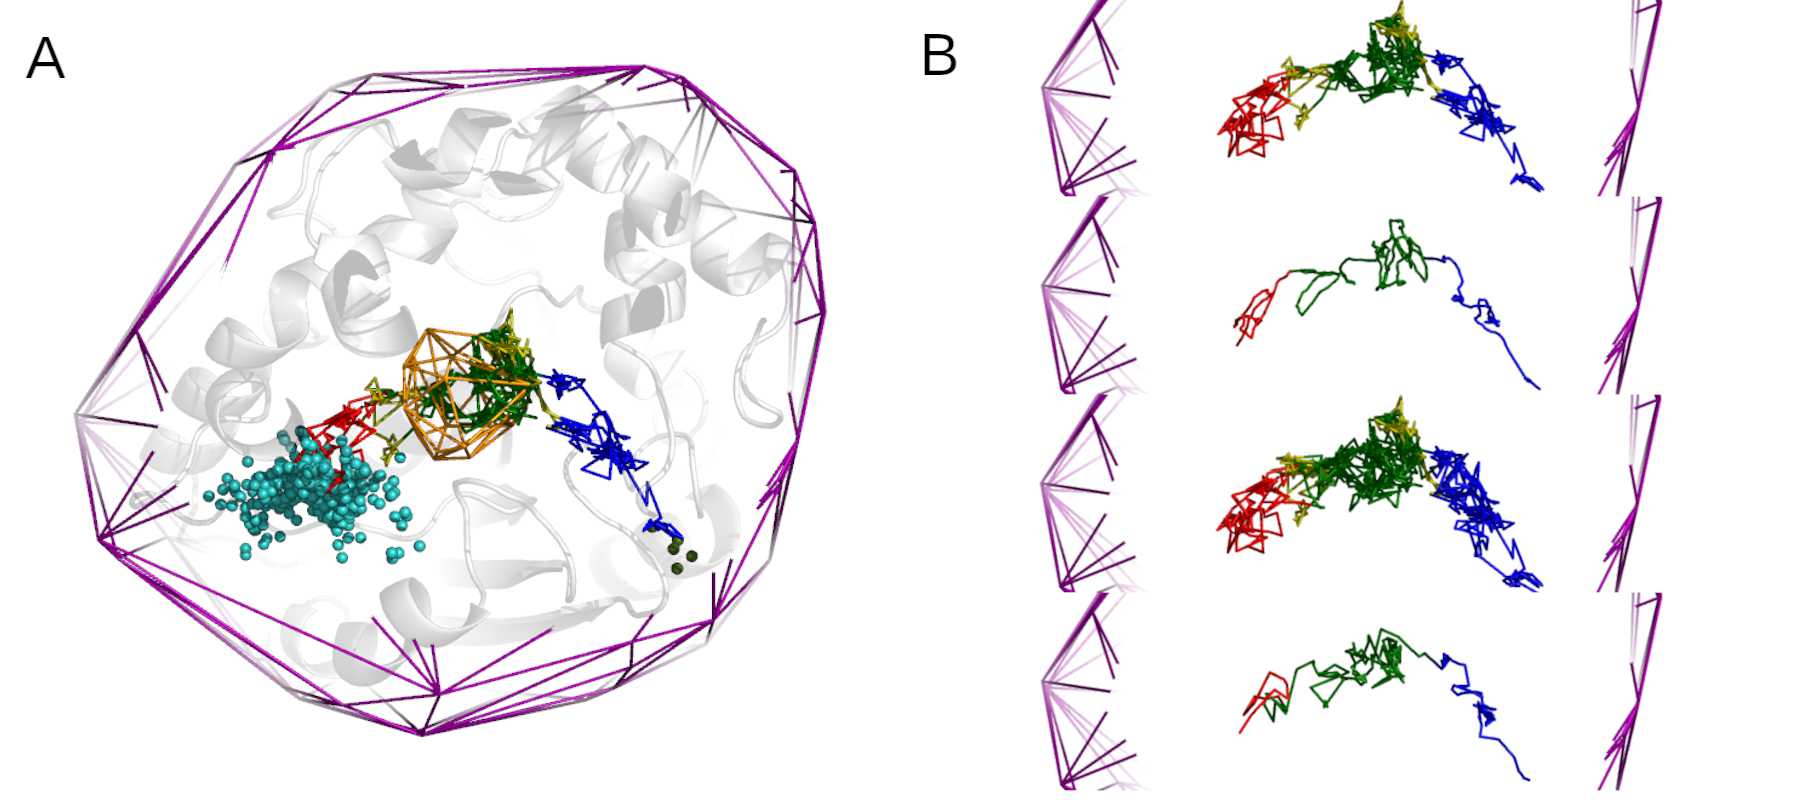
\includegraphics[width=\textwidth]{dictionary.png}
\caption{A graphical representation of terms used during AQUA-DUCT analysis: A) \emph{Scope}, \emph{Object}, cluster, inlet, and an example of a path, and B) selected single raw path, selected single smooth path (the same one as the raw one, but smoothed), all paths between \texttt{cluster\_1} and \texttt{cluster\_2}, and master path \texttt{1\_2}.}
\label{Dict}
\end{figure*}

\begin{itemize}
\item \textbf{\textit{valve}} is a driver that uses \textit{aquaduct} module to perform analysis of trajectories of selected residues in MD simulation.
\item \textbf{\textit{pond}} is a driver that uses \textit{aquaduct} module to perform further analysis of results from \textit{valve} calculations.
\item \textbf{\textit{kraken}} is a small application that helps to gather and visualize all quantitative results from AQUA-DUCT.
\item \textbf{\textit{Configuration file}} is a text file containing all necessary information needed to launch the AQUA-DUCT calculations. It can be prepared with AQUA-DUCT GUI Valve Configurator or it can be prepared with a template file that can be printed by \textit{valve}.
\item \textbf{\textit{Object}} is an area of greatest interest, only molecules which passed through \textit{Object} are traced. \textit{Object} should define residues to trace and spatial boundaries of the \textit{Object} site. The purpose of this space is to limit the number of tracked molecules to pathways of particular interest - this means gathering molecule movement data only relating to a particular space in the macromolecule, and by consequence, a pathway.
\item \textbf{\textit{Scope}} is an area within the analysed system inside which selected molecules should be traced. \textit{Scope} can be defined in two ways: as \textit{Object} but with broader boundaries or as the \href{https://tunneling-group.github.io/aqua-duct/valve/valve_manual.html?highlight=convex\%20hull#convex-hulls-of-macromolecule-atoms}{convex hull} of selected molecular object, e.g., protein.
\item \textbf{\textit{Inlet}} is a graphical representation of the point in which a traced molecule entered or left the defined \textit{Scope}. Inlets are then grouped into clusters.
\item \textbf{\textit{Cluster}} is a collection of inlets that represents entry/exit location to/from the system which was simulated during the MD simulation. In AQUA-DUCT, clusters simply mean particular tunnels entry/exits.
\item \textbf{\textit{Traced molecules}} are user-defined type of molecules (such as water molecules, cosolvents, ligands or other small molecules) which passed through the defined \textit{Object} during the simulation time and therefore are traced and further analysed.
\item \textbf{\textit{Traceable residues}} is a list of all traced residues.

\item \textbf{\textit{Path}} is a visualization of a traced molecule's trajectory within the defined \textit{Scope} and \textit{Object}. Paths are coloured as follows:
red - traced molecule entered \textit{Scope} and is heading to the \textit{Object}
green - traced molecule is in the \textit{Object}
yellow - traced molecule left the \textit{Object}, entered the \textit{Scope} and then again entered the \textit{Object}
blue - traced molecule left the \textit{Object} and is heading to leave the \textit{Scope}
\item \textbf{\textit{Raw path}} is an object created for each of the \textit{Traceable residues} which stores frames in which a residue is in \textit{Scope} or \textit{Object}; in PyMOL visualization it is a graphical representation of an actual trajectory of a particular tracked molecule.
\item \textbf{\textit{Smooth path}} is a path that has been smoothed using one of the available methods: Savitzky-Golay filter, Window smoothing (default method), Distance Window smoothing, Active Window smoothing, Max Step smoothing, Window over Max Step smoothing, Distance Window over Max Step smoothing, Active Window over Max Step smoothing; in PyMOL visualization it is a graphical representation of a smoothed trajectory of a particular tracked molecule. Smooth paths can (and are recommended to) be used for energy profile calculations.
\item \textbf{\textit{Master path}} is a representative of a group of paths that begin and end in a particular inlets cluster shown in PyMOL representation. 
\item \textbf{\textit{Passing paths}} are traces of molecules that entered the \textit{Scope} but did not visit the \textit{Object}.
\item \textbf{\textit{AutoBarber}} is a procedure which trims paths down to the  approximated surface of the macromolecule or other molecular entity defined by the user. The trimming is done by creating collection of spheres that have centers at the ends of paths and radii equal to the distance from the center to the nearest atom of molecular entity defined by the user. Next, parts of raw paths that are inside these spheres are removed and separate paths are recreated.
\item \textbf{\textit{Pockets}} represent the space of a particular macromolecule which were visited by tracked molecules during the simulation time.
\item \textbf{\textit{Hot-spots}} are defined as points in 3D space characterised by the highest local density of the traced molecules (most often solvent molecules). These are locations where water or other solvent molecules are "attracted" by beneficial interactions with nearby amino acids, or where they are trapped in the macromolecule's interior. In both cases, hot-spots may indicate regions of particular importance for macromolecule's function and/or drug design.
\item \textbf{\textit{Energy profile}} is the local free energy value estimated using calculated density of tracked molecules. Estimation of free energy is done according to Boltzmann inversion. Similar method was used in \cite{Rao2017} paper.
\item \textbf{\textit{Cosolvent}} is defined in this tutorial as any low molar mass chemical compound that may be (at least moderately) mixed with water. Cosolvents may act as small molecular probes, similarly as water molecules, penetrating the internal structure of the protein. Since cosolvents have different physico-chemical properties than water molecules, it allows the user to analyse different properties and penetrate different regions of the analysed macromolecule.
\end{itemize}

\subsection{Tutorial 1: Basic solvent transportation analysis}
For all Tutorials published here the authors have prepared three samples of training data. They also encourage the users to create 
separate directories for particular data sets. Therefore, the authors recommend the users to navigate to the directory they would like to use as a working directory and create a \texttt{Tutorial} directory. Within, it is recommended to create a directory for this (and a number of others using the same data) tutorial. 

For this tutorial, the user should create \texttt{1\_basic\_analysis} working directory. Here, the user will use a set of MD simulations data
- \href{http://www.aquaduct.pl/user-guide/}{sample data \#1} which comprises of topology and trajectory files of mouse soluble epoxide hydrolase in a water box.

To launch AQUA-DUCT GUI Valve Configurator the user should use the command:
\begin{lstlisting}
valveconfig_run
\end{lstlisting}
Within the GUI Valve Configurator one can either prepare a configuration file from scratch or load an existing one. 
For this tutorial, select the Easy configuration level. The Easy level of the GUI Valve Configurator consists of 3 tabs that correspond to the essential steps of AQUA-DUCT calculations: \textit{Initial step}, \textit{Clustering} and \textit{Visualization}.
Firstly, in the \textit{Initial step} tab, a topology file and trajectory files must be provided: this can be done either through file selection menu ("Load") or through inputting a path to the file. The path can be either absolute or relative to the directory from which the program was launched. AQUA-DUCT supports multiple topology and trajectory file formats including XPDB, MMTF, PRMTOP, TOP, PSF, PDBQT, MOL2, PQR, TRP, CRD, PARM7, GRO, XYZ, PDB for topology and CRD, MDCRD, XPDB, DCD, NC, NetCDF, TRJ, CRDBOX, TRZ, GRO, TRR, PDB, LAMMPS, MMTF, RESTRT, XTC for trajectory formats. For more information on available files formats please look at \href{https://www.mdanalysis.org/docs/documentation_pages/topology/init.html}{MDAnalysis documentation - Topology} and \href{https://www.mdanalysis.org/docs/documentation_pages/coordinates/init.html}{MDAnalysis documentation - Trajectory}. Also, setting the \texttt{cache} option by providing a path to a cache directory is advised, where AQUA-DUCT will store essential files for the calculations.

The first tutorial aims to explain how to access information about the space which is penetrated by solvent molecules. During the course of molecular dynamics simulations, small molecules, such as solvent molecules, ligands or ions, are able to penetrate the macromolecule's cavities, and therefore they are used by AQUA-DUCT as a molecular probe. Each small molecule may enter and/or leave the macromolecule's interior many times, therefore for the clarity of the results, AQUA-DUCT filters the flow of analysed small molecules by applying two regions of particular interest. The first region of interest is called the \emph{Scope} and it represents the region within which small molecules are traced. The second region, the \emph{Object}, represents the cavity of particular interest, such as the enzyme's active site, cofactor's cavity, or some other cavity of the user's interest, which the small molecule must visit to be traced. Therefore it is very important to place the \emph{Object} within the \emph{Scope}. 

Since this tutorial is focused on tracking water molecules inside the whole protein, the \textit{Scope} needs to be set to \texttt{protein}. The  definition  of \textit{Object} is somehow more complicated and consists of two essential pieces of information: the name of tracked molecules (e.g., water, other solvent, ions, or combination of several different small molecules) and the space which they must visit to be tracked, e.g., the active site, binding cavity or some other pocket. To learn more about the selection queries please see the \href{https://www.mdanalysis.org/docs/documentation_pages/selections.html}{MDAnalysis documentation - Selection} section. In this tutorial the \emph{Object} definition will be set as water molecules (\texttt{resname WAT}) within 6 Å sphere of the centre of geometry defined by active site amino acids (residues 99, 147, 231, 261 and 289) which approximates the active site pocket:
\begin{lstlisting}
(resname WAT) and (sphzone 6.0 (resnum 99 or resnum 147 or resnum 231 or resnum 261 or resnum 289))
\end{lstlisting}

When AQUA-DUCT tracks a molecule, information about that molecule is stored as a \emph{path}. A \emph{path} shows where the molecule of interest has entered the \emph{Scope}, visited the \emph{Object} (or left the Object and entered it again etc.) and left the \emph{Scope}. If the molecule of interest have entered and left the protein, the beginning and the end of each path are marked by inlets. Later, during the clustering stage, those inlets are grouped into clusters, which will have individual ids. Within \texttt{valve} results, paths are typically identified by its starting and ending point, using cluster ids in an start-finish format (e.g 1-1, 2-1 or 2-N). Sometimes the path could end inside the area of interest, i.e. inside the \emph{Scope}. Some paths may also begin inside the \emph{Scope}, depending on starting simulation conditions. Such path starting and ending points are marked as N. This will be discussed further, during the analysis stage. As a rule of thumb, it is desirable for inlets (and by extension, path starting and ending points) to stay on the protein’s surface. This way they can be effectively used to mark the tunnels’ entrances. This, however is not always the case right after second stage of \emph{valve} calculations, so for this purpose \emph{AutoBarber} is used to trim the pathways so they align with protein surface. AQUA-DUCT uses the \href{https://tunneling-group.github.io/aqua-duct/valve/valve_manual.html?highlight=paths#convex-hulls-of-macromolecule-atoms}{ConvexHull} approximation to describe the protein’s surface. As a consequence of that the inlets usually flow beyond the protein’s surface and are widely dispersed. \emph{AutoBarber} cuts the paths to fit them into the protein’s surface. The user can define the level of path trimming. Typically when \textit{AutoBarber} is set to \texttt{protein}, the paths will be longer than when it is set \texttt{backbone}, while if it is set to \texttt{name CA} the paths will be the shortest. For more detailed information please see the \href{http://www.aquaduct.pl/trimming-paths/}{Trimming paths Tutorial} on the AQUA-DUCT website.

In the first tab, \textit{Initial}, the user needs to set the paths to their topology and trajectory files, then define the \emph{Scope} and \emph{Object}, and set the \textit{Auto Barber} option to \texttt{protein}. Then, the user can switch to \textit{Clustering} tab.

Possibly the most challenging part of AQUA-DUCT calculations involve clustering the inlets. Typically it is desired to group entering molecules by the tunnel entrance they enter the protein through. If the protein has more tunnels we can separate them, and see how often each of them is used. The AQUA-DUCT provides user full flexibility how to group the clusters together to answer each possible question focused on solvent flow through the protein interior.  
For first-time use the authors recommend using the \texttt{barber} method, and setting \emph{auto\_barber} to \texttt{protein}, and leave the other options default. This method will provide the user with the first glance of the system of interest and the water paths network. The \emph{AutoBarber} procedure works here in a similar manner that it is during in the previous step, but that does not mean that the same set of settings needs to be used. The available combination of \emph{AutoBarber} settings for trimming paths are available at the AQUA-DUCT website in the \href{http://www.aquaduct.pl/trimming-paths/}{Trimming paths Tutorial}.

The last step before finally running AQUA-DUCT is the visualization. This is done from the \textit{Visualize} tab. Here, the user defines specifically what aspects of calculations they want to visualize. Since the  molecule, \emph{Scope}, \emph{Object} and clusters are subjects of this analysis, they should be selected. Since this part of the tutorial is focused on different types of paths, the user is encouraged to choose all of the available options. It is recommended to change the \emph{Object} definition to \texttt{(resname *) and (sphzone 6.0 (resnum 99 or resnum 147 or resnum 231 or resnum 261 or resnum 289))} replacing the small molecules type by an asterisk (*) for the visualization clarity.

\begin{Checklists}
\begin{checklist}{TIP}
\textbf{PyMOL visualization files}

The visualization file (PyMOL session) can be really large, when the user wants to include all the available information (even over 1GB). Therefore, in the first round of analysis, the authors recommend not to include the raw paths option. However, the analysis of the raw paths could be necessary, when the user is not sure if neighbouring clusters mark different tunnels’ exits, or if they can be merged.
\end{checklist}
\end{Checklists}

With the configuration ready, the configuration file should be saved (\emph{File > Save As}). Once it is saved, the user can begin through selecting \emph{Run > Valve}, within the Run window. It is also possible to select the maximum number of threads used (leaving the option empty uses all available threads) and launch options. It is recommended for the user to use the \textit{Debug absolute file path} to ensure that a log file will be created and all the information on the calculations will be saved to this file. Once the \textit{Config absolute file path} and \textit{Debug absolute file path} are provided, the user should see in the Run Valve window a below information: 
\begin{lstlisting}
valve_run -c /home/username/Tutorial/1_basic_analysis/config.txt --debug-file /home/username/Tutorial/1_basic_analysis/aq.log
\end{lstlisting}
where \texttt{/home/username/Tutorial/1\_basic\_analysis} means the actual working directory where the user is running this tutorial and the sample data set.
If the option \texttt{-{}-debug-file} is used, AQUA-DUCT will create a file that contains a record of all AQUA-DUCT calculations and information about possible errors. 
Now the user can press "Run" button to begin the calculations. 

After the AQUA-DUCT calculations finish (such calculations take approx. 8 minutes on an Intel Core i7-4790 CPU @ 3.60 GHz machine), the user will get some files which store results from each stage of the analysis:

\begin{enumerate}
    \item dump files (\texttt{1\_traceable\_residues\_data.dump}, \texttt{2\_raw\_paths\_data.dump}, \texttt{3\_separate\_paths\_data.dump}, and \texttt{4\_inlets\_clustering.dump}) containing essential data for further AQUA-DUCT analysis steps
    \item \texttt{5\_analysis\_results.txt}, \hfill and \newline \texttt{analysis\_results.txt.csv} files that contain contextualized data from the analysis
    \item \texttt{6\_visualize\_results.py}, \hfill and \newline \texttt{6\_analysis\_results.tar.gz} files used to generate data visualization.
\end{enumerate}

AQUA-DUCT handles the visualization of the results by using PyMOL. The easiest way to preview the results is to use the \texttt{6\_visualize\_results.py} script.
The script for visualization has a set of arguments that allows the user to decide which items they want to see in their PyMOL session, change colours of some objects or automatically save their generated visualization as a PyMOL session (Figure \ref{Tut1.1}), among others. All functionality can be viewed using:
\begin{lstlisting}
python 6_visualize_results.py --help
\end{lstlisting}
Furthermore, all usable arguments are listed within \href{https://tunneling-group.github.io/aqua-duct/valve/valve_manual.html?highlight=visualize\%20results#visualization}{documentation}.

To launch the script use:
\begin{lstlisting}[columns=fullflexible]
python 6_visualize_results.py --keep 'molecule cluster scope object raw'  --discard  'master io all paths'
\end{lstlisting}
The user should pay particular attention to copying commands from these tutorials to the command line, since they can unintentionally copy different characters than they seem to appear in the text.

\begin{figure}[htp!]
\centering
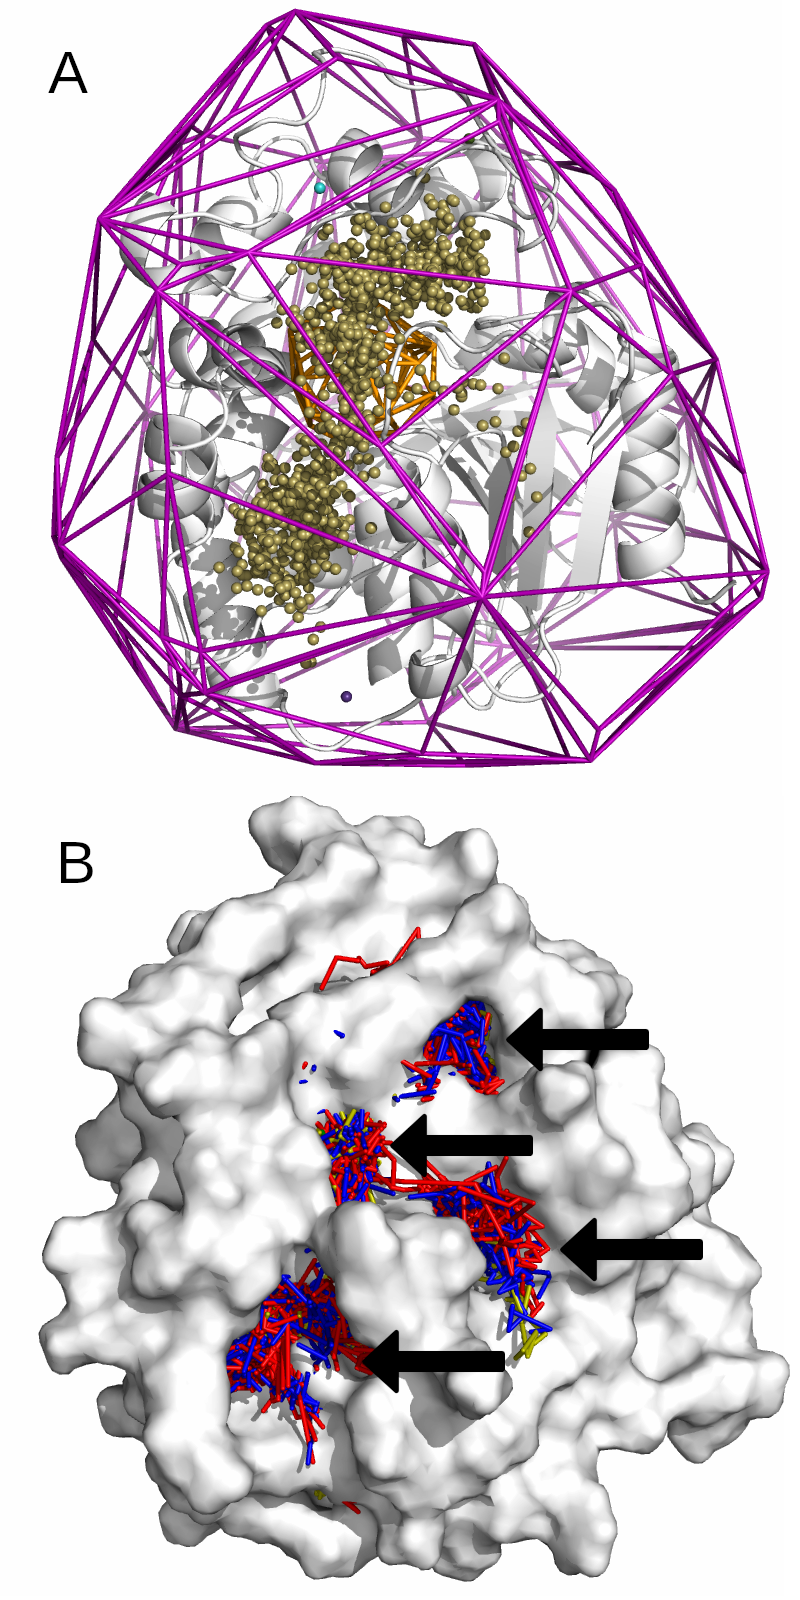
\includegraphics[width=0.5\textwidth]{Tut1.1.png}
\caption{AQUA-DUCT visualization results. A) The cluster of inlets view. B) The visualization of the raw paths. The macromolecule is shown as white surface, the inlets are shown as small spheres, and the raw paths are shown as lines colour-coded as follows: red - parts of paths that entered the macromolecule, blue - parts of paths that left the macromolecule, green - parts of paths that remained in the \textit{Object} region, and yellow - parts of paths that left the \textit{Object}, wandered around the protein's interior and went back to the \textit{Object}.}
\label{Tut1.1}
\end{figure}

Using this command, the user is omitting the smooth paths and many more items AQUA-DUCT is capable of visualising. This visualization will be used to verify how appropriate clustering results are - using all visualization options can potentially take more time than needed and as such for this purpose \texttt{-{}-keep} and \texttt{-{}-discard} options are used to only keep elements that are of interest: the molecule, \textit{Scope}, \textit{Object}, clusters and raw paths. While \texttt{-{}-keep} works as one would expect, only keeping specified elements and discarding the others, using \texttt{'raw'} argument will also keep such elements as \texttt{'raw\_master\_paths'} or \texttt{'all\_raw\_in'}. For this reason \texttt{-{}-discard} option is also used as shown. 

This part of the tutorial ends with looking at the visualization of the AQUA-DUCT results (Figure \ref{Tut1.1}) and assessing the quality of the conducted clustering of inlets. The purple shape represents the \emph{Scope} and the orange stands for the \emph{Object}, inlets are shown as small spheres, and only raw paths are shown for the picture clarity. When examining the correctness of clustering method used, it is important to focus on how the pathways and inlets are positioned on the protein's surface. The clusters of inlets should be disabled in PyMOL and only the raw paths should be used to identify the potential entrances to the \textit{Object}. The red (Incoming) and blue (Outgoing) parts of paths represent the flow of the traced molecules, and therefore their positions on the protein's surface reflect the shape and the size of the potential entrances/exits, as well as their connection with the \textit{Object} cavity. Therefore, they also reflect the shape and size of tunnels leading to the active site. In Figure \ref{Tut1.1} there are four visible entries to the active site pocket (marked with arrows), each of them picture a particular tunnel connecting the enzyme's active site with the environment. To analyse how often the identified tunnels are used, a proper clustering of the inlets is required. The position of the inlets clusters should overlap with the entries/exits to the protein. Tutorial~2 shows how to conduct multi-level clustering using AQUA-DUCT's GUI Valve Configurator to properly divide the big \texttt{cluster\_1} into four smaller clusters, reflecting the positions of entrances/exits to the enzyme's active site.

\subsection{Tutorial 2: Advanced solvent transportation analysis: multi-level clustering and visualization tips}

The previous tutorial ends with the first visualization of the AQUA-DUCT results and the user realising that the default clustering method is not always sufficient, and has to be adjusted to provide a detailed picture of the solvent flow between different tunnels entries. For the purposes of Tutorials 1-3, the authors prepared sample data \#1 of an enzyme which entrances/exits to its active site are close to each other and change their shape and size substantially during the course of the MD simulation, so that the default method of clustering merge them into one cluster. Therefore, to divide them according to their position on the protein's surface, it is necessary to examine the raw paths, which provide information about the space accessible to tracked molecules and allow to detect locations of tunnels division and separate entrances. The next step of such an analysis is the clustering of the identified inlets, in such a way, that they will occupy the same space on the protein's surface as the red (Incoming) and blue (Outgoing) parts of paths divided by spaces inaccessible for the tracked molecules. In this case, the user needs to know how to use different clustering algorithms, but first they need to understand how to identify a potential entry/exit to the particular cavity of interest. It should be noticed that in some cases, for example when the entrances/exits to the active site or a cavity of particular interest are separated, the user is not going to need such a complex multi-level clustering approach and the default clustering method should be sufficient. Also flexibility of the clustering methods allows the user to join together any clusters of interest and by such an approach examine for example transportation of molecules in particular direction by multiple tunnels.

Figure \ref{Tut1.1}B shows the protein's surface and only raw identified paths of the traced molecules. To obtain such results the user needs to type in the command line:
\begin{lstlisting}[columns=fullflexible]
python 6_visualize_results.py --keep 'molecule cluster scope object raw' --discard 'master io all paths smooth'
\end{lstlisting}
and show the protein as surface using PyMOL options.

The user should now be able to see four regions where the raw paths are entering and/or leaving the protein's surface (marked with arrows in Figure \ref{Tut1.1}B. To be able to analyse each entrance/exit separately, the user need to divide the big \texttt{cluster\_1} into four separate clusters indicating particular entries. Then, they will be able to access detailed information on the direction of small molecules flow, the length of pathways passing through each entry, the possibility of such a passage, etc. In this tutorial the user will use the GUI Valve Configurator to modify their first configuration file in order to add some more clustering steps. 

Since now the user wants to repeat only the clustering stage, they do not have run the calculations from the three previous steps again. The authors are aware that in some cases, such as long simulations of a protein which is visited by a large number of small molecules, the calculation may take a while. Therefore for every stage of the AQUA-DUCT calculations there is an \textit{execute} option which can be set to \texttt{runonce}, \texttt{run} and \texttt{skip}. The default setting here is \texttt{runonce} which allows AQUA-DUCT to search for a previously generated \texttt{.dump} file and load the results from the \texttt{.dump} file. When it is set to \texttt{run}, the calculations are run, overriding the previously generated \texttt{.dump} files. If it is set to \texttt{skip} the calculations are skipped and if the corresponding \texttt{.dump} file exists, it is loaded. However, it is recommended in this step to create a new directory to copy the previously generated files.

To keep all the data and avoid overwriting the files in next runs of calculations, we recommend the user to copy the \texttt{4\_inlets\_clustering\_data.dump}, \texttt{5\_analysis\_results.txt}, \texttt{5\_analysis\_results.txt.csv}, \texttt{6\_visualize\_results.py}, and \texttt{6\_visualize\_results.tar.gz} files from the previous run and store them in a separate directory, called for example \texttt{run\_1}. After each calculations the user is encouraged to create a new directory in which they will keep the previously generated files.

First, the user needs to type in the command line:
\begin{lstlisting}
valveconfig_run
\end{lstlisting}
and then use the \textbf{Load Config} button to browse files and select the previously generated \texttt{config.txt} file, chose the Normal level of the configuration file editing and click \textbf{Forward} button. Now they should see five tabs: \textit{General options}, \textit{Tracking}, \textit{Inlets clustering}, \textit{Clustering}, and \textit{Visualization}.

A new recursive clustering section can be added in the fourth tab, \textit{Clustering}, by clicking on the \textbf{Add clustering section} button. Above this button, a \textit{Recursive clustering} option is visible. The value of this option (default being "clustering") points to the name of the next clustering section which should be added next. After clicking the button, the user will see another box titled "Recursive clustering" inside which the first field is \textit{Name}. This is the name that the first \textit{Recursive clustering} field should point to - their values should be the same name. The \textit{Name} of a newly added section will be "clustering0" by default. Here, the first \textit{Recursive clustering} field needs to be adjusted accordingly to "clustering0". This is indicating that clustering section of this name is to be executed as part of the recursive clustering. Should the user add more recursive clustering sections, each previous recursive clustering sections \textit{Recursive clustering} field should point to (contain) the \textit{Name} of the next one, creating a "chain". Now having a newly added recursive clustering section, the user should select the \emph{birch} clustering method and set \emph{Cluster number} to \texttt{4} in order to divide the biggest cluster into 4 smaller pieces. Then they should set \emph{Recursive threshold} to \texttt{>0.9} to define the size of the cluster to be divided.

\begin{Checklists}
\begin{checklist}{TIP}
\textbf{Clustering methods}

There is more than one way to divide one cluster into four smaller pieces. There are several clustering methods implemented in AQUA-DUCT, such as Barber, Meanshift, Birch, Kmeans, DBSCAN, and AffinityPropagation. The user is encouraged to try different methods of clustering to find their own method of solving this clustering task. To learn more about the clustering methods please see \href{http://www.aquaduct.pl/clustering/}{Clustering tutorial} on the AQUA-DUCT website.
\end{checklist}
\end{Checklists}

\begin{Checklists}
\begin{checklist}{TIP}
\textbf{Editing configuration file manually}

If the user wishes to proceed with preparing configuration file without using the GUI Valve Configurator, when adding recursive clustering keep in mind that in configuration file, aforementioned \textit{Name} field of a recursive clustering section is not an option within the \texttt{clustering} section, it is a name of a new section that the user would add manually instead.
\end{checklist}
\end{Checklists}

The \emph{Recursive threshold} needs to be set to a float value which reflects the size of a particular cluster relative to the number of all identified inlets. The information of each cluster's size is stored in the \texttt{5\_analysis\_results.txt} file in the \emph{Clusters summary - inlets} table. In the case of the \texttt{cluster\_1} which consists of 1117 inlets, with the total number of identified inlets equal to 1120, setting it \texttt{>0.9} is correct.

To speed up the calculations, the user needs to change \textit{execute} option to \texttt{run} inside the \textit{Inlets clustering} tab to ensure that the calculations will start from the clustering stage, and AQUA-DUCT will load the three previously generated \texttt{.dump} files. As the user may notice, the value of the \emph{Max level} option had changed to 1. This value is equal to the number of the recursive clustering sections added by the user and it is automatically set by the GUI Valve Configurator. When the user plans not to use the GUI Valve Configurator, they need to remember to set the \texttt{max\_level} option in the \texttt{[inlets\_clustering]} section in the configuration file manually. Now the user can save the modified configuration file as \texttt{config2.txt}

To run the AQUA-DUCT calculations, the user should type in the command line:
\begin{lstlisting}[columns=fullflexible]
valve_run -c config2.txt --debug-file aq2.log
\end{lstlisting}

During the AQUA-DUCT run, the user will see a clustering history tree which shows how the clusters were divided.
\begin{lstlisting}
Clustering history:
all-+ {size: 1120; BarberCluster}
    1-+ {size: 1117; Birch}
    | 5 {size: 222}
    | 6 {size: 379}
    | 7 {size: 291}
    | 8 {size: 225}
    2 {size: 1}
    3 {size: 1}
    4 {size: 1}
\end{lstlisting}

\begin{figure}[ht!]
\centering
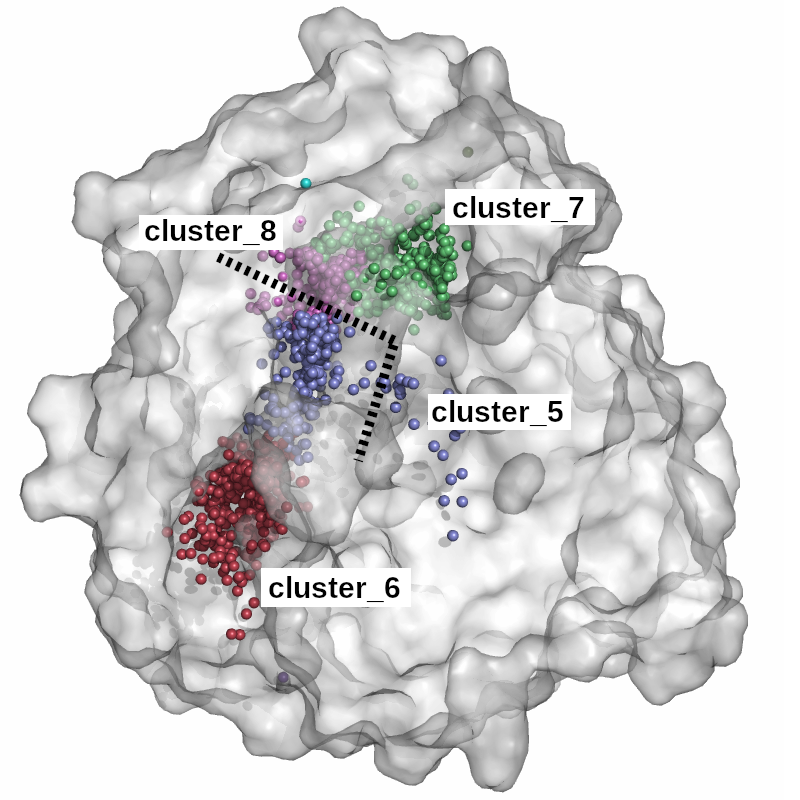
\includegraphics[width=0.5\textwidth]{Tut2.1.png}
\caption{AQUA-DUCT visualization results after the first run of multi-level clustering approach. The one big cluster is divided into four parts using the \texttt{birch} method: \texttt{cluster\_5} - lightpurple spheres, \texttt{cluster\_6} - red spheres, \texttt{cluster\_7} lightgreen, and \texttt{cluster\_8} - pink spheres. The second run of the clustering requires division of two clusters which is marked with dashed lines.}
\label{Tut2.1}
\end{figure}

After the calculations finish (on an Intel Core i7-4790 CPU @ 3.60 GHz machine these calculations take approx. 5 minutes), type the command below to visualize only clusters of inlets, the macromolecule, the \emph{Object} and the \emph{Scope}:
\begin{lstlisting}[columns=fullflexible]
python 6_visualize_results.py --keep 'molecule cluster scope object'
\end{lstlisting}

The biggest cluster was divided into four smaller clusters, but they do not reflect the entrances/exits to/from the active site cavity. However, by applying small changes to two of the clusters, namely \texttt{cluster\_5} and \texttt{cluster\_8}, the user will be able to achieve their goal (Figure \ref{Tut2.1}). The strategy proposed by the authors is as follows: two clusters need to be divided in halves, namely \texttt{cluster\_5} and \texttt{cluster\_8}. From the resulting clusters formed by the division of \texttt{cluster\_5}, the smallest one will become the cluster reflecting the side entrance/exit to the enzyme's active site and the second one will be the part of the gorge cluster between clusters \texttt{cluster\_6} and \texttt{cluster\_7}. From the resulting clusters from the division of \texttt{cluster\_8}, one part will be incorporated into \texttt{cluster\_7} and the other part will be joined with the gorge part of \texttt{cluster\_5}. 

The user needs to once again launch the GUI Valve Configurator by typing in their command line:
\begin{lstlisting}
valveconfig_run
\end{lstlisting}
and once again load the previously generated \texttt{config2.txt} file, select the Normal level of the configuration file editing and hit \textbf{Forward} button. In the \textit{Clustering} tab add another clustering section by clicking on the \textbf{Add clustering section} button. Then, in the newly generated "Recursive clustering" box, the \textit{Name} field will be set to \texttt{clustering1}. Here the user needs to remember to change the \textit{Recursive clustering} field of the last clustering section (here that would be \texttt{clustering0}) to this generated name (that is \texttt{clustering1}). Now in the \texttt{clustering1} the user needs to set the clustering method to \emph{birch} and set \emph{Cluster number} to \texttt{2}. Now the \emph{Recursive threshold} should be set to \texttt{<0.25} to ensure that both \texttt{cluster\_5} (size of 222 inlets, which reflects 0.2 of all identified inlets) and \texttt{cluster\_8} (size of 225 inlets, which reflects 0.2 of all identified inlets will be divided into 2 pieces. The last step will require joining clusters.
Now the user needs to save the modified configuration file as \texttt{config3.txt} and run AQUA-DUCT calculations:
\begin{lstlisting}[columns=fullflexible]
valve_run -c config3.txt --debug-file aq3.log
\end{lstlisting}
During the AQUA-DUCT run the user will see a clustering history tree which shows how the clusters were divided.
\begin{lstlisting}
Clustering history:
all-+ {size: 1120; BarberCluster}
    1-+ {size: 1117; Birch}
    | 5-+ {size: 222; Birch}
    | | 9 {size: 199}
    | | 10 {size: 23}
    | 6 {size: 379}
    | 7 {size: 291}
    | 8-+ {size: 225; Birch}
    |   11 {size: 117}
    |   12 {size: 108}
    2 {size: 1}
    3 {size: 1}
    4 {size: 1}
\end{lstlisting}

After the calculations finish (on an Intel Core i7-4790 CPU @ 3.60 GHz machine these calculations take approx. 5 minutes), type the command below to visualize only the clusters of inlets, the macromolecule, the \emph{Object} and the \emph{Scope}:
\begin{lstlisting}[columns=fullflexible]
python 6_visualize_results.py --keep 'molecule cluster scope object'
\end{lstlisting}

\begin{figure}[ht!]
\centering
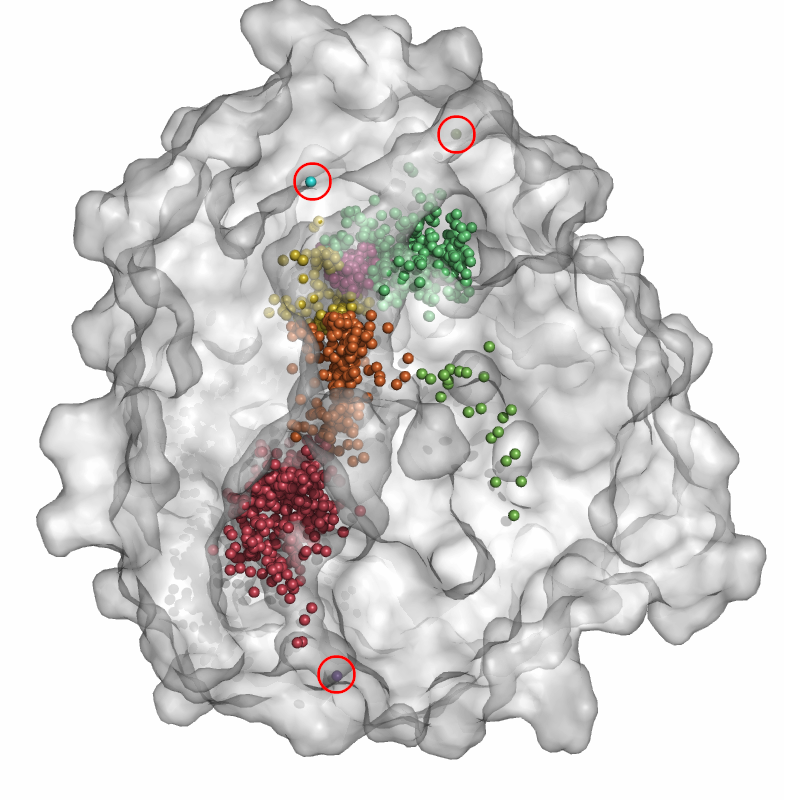
\includegraphics[width=0.5\textwidth]{Tut2.2.png}
\caption{AQUA-DUCT visualization results after the second run of multi-level clustering approach. Two of the clusters were divided into two parts and now the user needs to join them according to the location of the tunnels entrances/exits. The small clusters containing one inlet which will be gathered in the next run into outliers cluster are marked by red circles.}
\label{Tut2.2}
\end{figure}

The user should be able to see nine clusters (Figure \ref{Tut2.2}), three of which consist of only one inlet, namely \texttt{cluster\_2}, \texttt{cluster\_3}, and \texttt{cluster\_4}. In the last step of clustering, the user will create an outliers clusters which will consist of all those inlets in order to keep the results more clear. They also need to join two clusters, namely \texttt{cluster\_7} and \texttt{cluster\_12}, and \texttt{cluster\_9} and \texttt{cluster\_11} to achieve the perfect overlap of the clusters of inlets with the entrances/exits to the active site cavity.

By \textit{outliers} the authors define inlets which represent rarely occurring passages, usually corresponding to the protein leakage or some other rare events. Such rare events can be useful for protein engineering, e.g. identification of potential pathway that can be opened to create fully functional tunnel \cite{Magdziarz2020,Brezovsky2016} or identification of cavities that can be used to reshape the binding site \cite{Mitusinska2018}.

For the last time the user needs to run the GUI Valve Configurator by typing in the command line:
\begin{lstlisting}
valveconfig_run
\end{lstlisting}
Then they need to load the previously generated \texttt{config3.txt} file, select the Normal level of the configuration file editing and hit \textbf{Forward} button. In the third tab, \textit{Inlets Clustering}, the user needs to set the \emph{Join clusters} option to \texttt{7+12 9+11} (please mind that there is no comma or a dot, only white space character) in the "Post Clustering Optimization" box. Please also tick the box next to the \emph{Renumber clusters} option to first join the selected clusters and then renumber them according to their sizes. To create an outliers cluster the user needs to change the \emph{Detect outliers} option to \texttt{Auto}, and set the \emph{Singletons outliers} to \texttt{1}. Setting \emph{Singletons outliers} to \texttt{1} will move the small clusters consisting of only one inlet to \texttt{cluster\_out}. As the user may also notice, the value of the \texttt{max\_level} option had changed to 2, reflecting the two additional recursive clustering sections which were added during the modification of the configuration file. 

Since the user is now reaching the final clustering which will successfully divide entries/exits of the analysed protein, they can additionally calculate relevant information like the volume and area of both the \textit{Object} and \textit{Scope}. For this, the user needs to select the \textit{Tracking} tab and in the "Calculate scope and object size" box, tick the option \textit{Calculate scope and object size} and set the definition of the \textit{Scope} and \textit{Object}; the \textit{Scope hull definition} should be set to \texttt{protein} and the \textit{Object convex hull} to \texttt{(resname *) and (sphzone 6.0 (resnum 99 or resnum 147 or resnum 231 or resnum 261 or resnum 289))}, repeating the \textit{Object} definition with the replacement of the molecule type (e.g., WAT) with an asterisk (*). As the user may see, the \textit{Cluster area} option is ticked automatically. It enables calculating the clusters’ areas with kernel density estimation method (KDE). To include such objects during the visualization, the user needs to tick the option \textit{Cluster area} in the \textit{Visualize} section as well. 

Now the user needs to save the modified configuration file as \texttt{config4.txt} and run it using the following command:
\begin{lstlisting}[columns=fullflexible]
valve_run -c config4.txt --debug-file aq4.log
\end{lstlisting}
During the AQUA-DUCT run, the user will see a clustering history tree which shows how the clusters were divided.
\begin{lstlisting}
Clustering history:
all-+ {size: 1120; BarberCluster}
    1-+ {size: 1117; Birch}
    | 5-+ {size: 222; Birch}
    | | 9 {size: 199; joined into: 14}
    | | 10 {size: 23; new nr: 4}
    | 6 {size: 379; new nr: 2}
    | 7 {size: 291; joined into: 13}
    | 8-+ {size: 225; Birch}
    |   11 {size: 117; joined into: 14}
    |   12 {size: 108; joined into: 13}
    2-+ {size: 1; |1| to outliers}
    | (0) {size: 1}
    3-+ {size: 1; |1| to outliers}
    | (0) {size: 1}
    4-+ {size: 1; |1| to outliers}
    | (0) {size: 1}
    0 {|1| to outliers; new size: 3; new nr: 0}
    13 {size: 399; made of 7+12; new nr: 1}
    14 {size: 316; made of 9+11; new nr: 3}
\end{lstlisting}

On an Intel Core i7-4790 CPU @ 3.60 GHz machine these calculations take approx. 5 minutes and 30 seconds. The user can eventually generate the final PyMOL session with all calculated paths and save them to the \texttt{clustering\_final.pse} file. The user does not have to use the option, since sessions can still be saved in PyMOL manually.
\begin{lstlisting}
python 6_visualize_results.py --save-session clustering_final.pse
\end{lstlisting}

\begin{figure}[ht!]
\centering
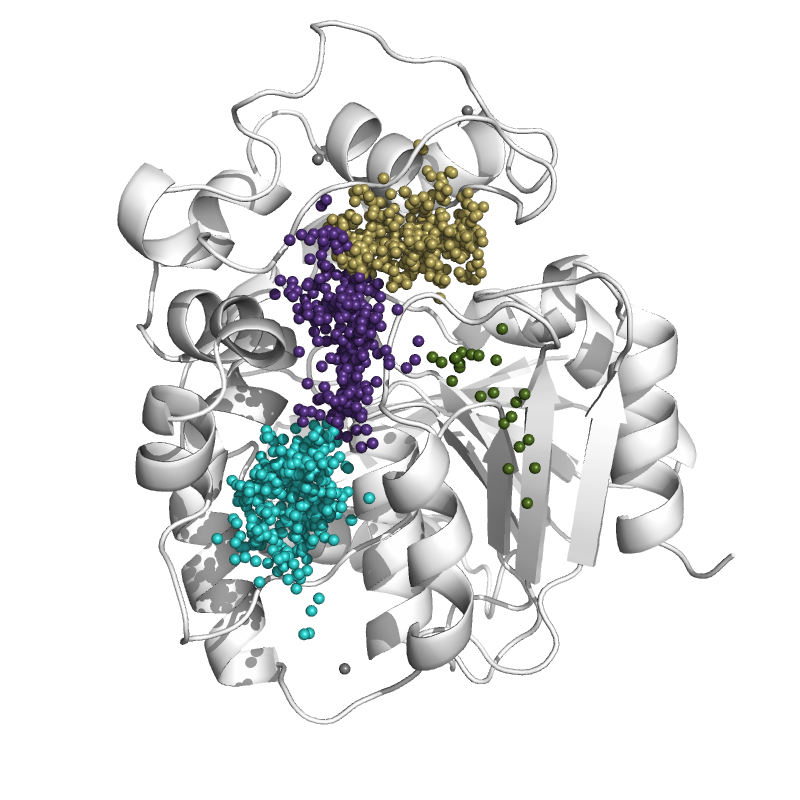
\includegraphics[width=0.5\textwidth]{Tut2.3.png}
\caption{AQUA-DUCT visualization results after the third run of multi-level clustering approach. The obtained clusters now overlap with the tunnels entrances/exits.}
\label{Tut2.3}
\end{figure}

The user will gain access to such paths as:
\begin{itemize}
\item raw paths
\item smooth paths
\item raw master paths
\item smooth master paths
\item smoothed raw master paths
\item all raw paths (as separate states in PyMOL session)
\item all smooth paths
\item raw paths IO (marks of the entrance and exit points for each path)
\item smooth paths IO
\item all "in" parts of raw paths
\item all "out" parts of raw paths
\item all "object" parts of raw paths
\item all "in" parts of smooth paths
\item all "out" parts of smooth paths
\item all "object" parts of smooth paths
\end{itemize}

The colour of a particular clusters of inlets is based on their ID, but it can be changed to any other colour defined in PyMOL using \texttt{-{}-force-color} option. The list of available colours can be found \href{https://pymolwiki.org/index.php/Color_Values#Interactive_menu_colours}{here}.

The user can change the colour of any chosen cluster of inlets. If they do not select a particular cluster of inlets, its colour will remain unchanged. To change the colours of four most common clusters of inlets, so they will correspond to those in Figure \ref{Tut2.4}, the user should type:
\begin{lstlisting}
python 6_visualize_results.py --force-color 'cluster_1 forest cluster_2 pink cluster_3 cyan cluster_4 limon'
\end{lstlisting}

\begin{figure}[ht!]
\centering
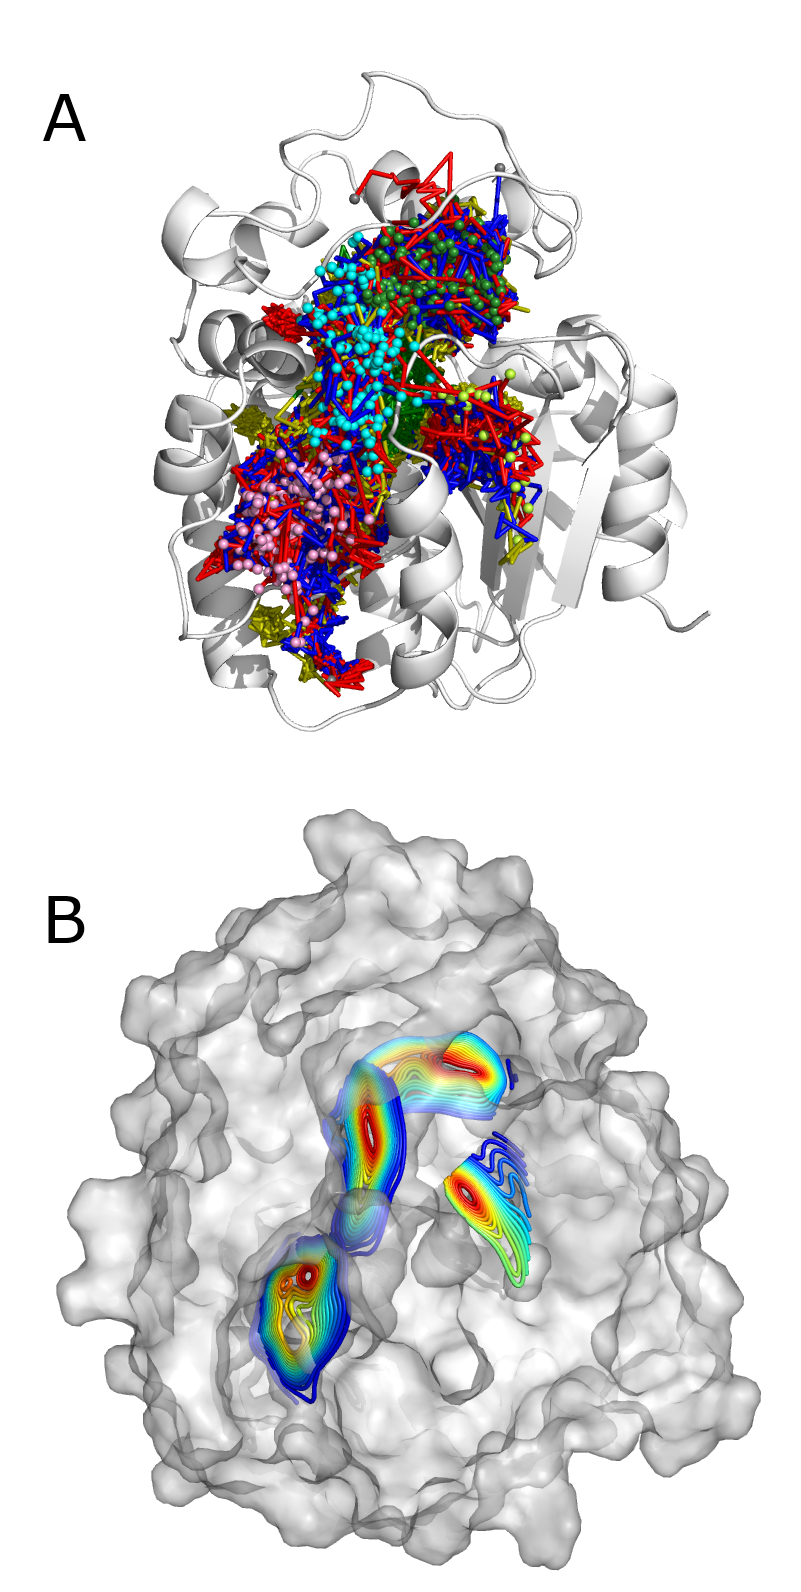
\includegraphics[width=0.5\textwidth]{Tut2.4.png}
\caption{AQUA-DUCT final visualization results after the last run of multi-level clustering approach. The obtained clusters now overlap with the tunnels entrances/exits, are coloured according to user-defined colours and all available paths are also shown. A) The visualization of clusters of inlets and raw paths. The macromolecule is shown as white cartoon. B) The visualization of clusters area. The macromolecule is shown as white, transparent surface, cluster areas are shown as coloured isolines.}
\label{Tut2.4}
\end{figure}

In this tutorial the user learned how to perform multi-level clustering using the GUI Valve Configurator tool. Running AQUA-DUCT calculations is possible also without using the GUI, only by editing the configuration file using the user's favourite text editor. This will be shown in the following tutorials. As it was mentioned, running multi-level clustering is useful in the case of a macromolecule which entrances/exits are not obviously separated. It should be noted that similar clustering results can be achieved by different clustering methods. The approach presented in this tutorial was chosen to demonstrate other useful options, such as \textit{Join clusters} and \textit{Singletons outliers}. To learn more about clustering methods implemented in AQUA-DUCT please check the \href{http://www.aquaduct.pl/clustering/}{Clustering tutorial} on the AQUA-DUCT website. The advanced clustering methods provide the user with an opportunity to flexibly merge and divide clusters according to the needs of the analysis. The user also learned how to use PyMOL visualizations to analyse the macromolecules's surface in order to identify the plausible entrances/exits to the cavity of particular interest.

\subsection{Tutorial 3: Quantitative analysis and visualization of the results}

In the previous two chapters, the user learned how much data can be acquired just with the visualization of the results in PyMOL. AQUA-DUCT calculations do not only allow to visualize the results, but also offer detailed  quantitative statistical data regarding the behaviour of tracked molecules, changes of the \textit{Scope} and \textit{Object} volume, etc. AQUA-DUCT includes a small and smart GUI application called \textit{kraken}, used to graphically visualize the aforementioned quantitative data. This chapter explains how to use it and presents results generated for the final results of AQUA-DUCT calculations in Tutorial 2. 

Statistical and quantitative results obtained with AQUA-DUCT are gathered in files \texttt{5\_analysis\_results.txt} and \texttt{5\_analysis\_results.txt.csv}. The user needs to provide \textit{kraken} these files in order to perform the analysis.

The first file, \texttt{5\_analysis\_results.txt}, consists of a set of 8 tables. A detailed explanation along with examples can be found in Supplementary figure 7 of the published article \cite{Magdziarz2020}. 
Table 1 \texttt{Clusters summary - inlets} consists of a summary of information about all inlets that form individual clusters.
Table 2 \texttt{Clusters summary - areas} constitute a summary of cluster areas.
Table 3 \texttt{Clusters statistics (of paths) probabilities of transfers} contains statistics of probabilities of separate paths transfers. Tables 4 and 5 represent statistics of paths' mean lengths in Å (table 4 \texttt{Clusters statistics (of paths) mean lengths of transfers}) and in number of frames of transfers (table 5 \texttt{Clusters statistics (of paths) mean frames numbers of transfers}). Tables 6 and 7 contain summary of mean lengths in Å (table 6 \texttt{Separate paths clusters types summary - mean lengths of paths}) and in number of frames of transfers (table 7 \texttt{Separate paths clusters types summary - mean number of frames of paths}) of paths according to the Cluster Types. Table 8 \texttt{List of separate paths and properties} consists of a list of all separate paths and their properties. 

The other file - \texttt{5\_analysis\_results.txt.csv} contains calculated frames-dependant parameters analysis comprising of one table where each row corresponds to one frame of the simulation. The table comprises two types of calculated values: number of traced paths, and \textit{Object} and \textit{Scope} sizes. The first column \texttt{\# frame} contains number of frame indexed from 0. Following columns contain information about specific types of paths that occur in the course of the simulation and number of these columns varies in files depending on number of clusters obtained in AQUA-DUCT calculations. For each frame, the numbers of traced paths are calculated for the following categories:
\begin{itemize}
\item Name of traced molecules: \texttt{amol} is used for all possible names.
\item Paths types: (\texttt{object} for standard paths, \texttt{passing} for passing paths) and \texttt{apaths} for all possible paths types.
\item Clusters and cluster types: \texttt{aclusts} is used for all possible clusters and \texttt{actypes} is used for all possible cluster types.
\item Part of paths: \texttt{walk} corresponds to any part of path and in case of passing paths only this category is used, \texttt{in}, \texttt{object}, \texttt{out} correspond respectively to incoming, object, and outgoing parts, and \texttt{in\_out} corresponds to sum of incoming and outgoing parts.
\end{itemize}
The column name can for example be \newline \texttt{amol\_apaths\_aclusts\_object}, which indicates object part of paths, all types of paths from all possible clusters. Another example is \texttt{amol\_apaths\_1:2\_in} which indicates incoming parts of paths of all possible path types that passed from \texttt{cluster\_1} to \texttt{cluster\_2}.

If one sets in configuration file in section \texttt{[analysis]} option \texttt{calculate\_scope\_object\_size} to \texttt{True}, the table will at the end contain four columns with information about the area of the \textit{Scope} in [Å\( \displaystyle ^{2}\)] (column \texttt{scope\_area}), the volume of the \textit{Scope} in [Å\( \displaystyle ^{3}\)] (column \texttt{scope\_volume}), the area of the \textit{Object} in [Å\( \displaystyle ^{2}\)] (column \texttt{object\_area}) and the volume of the \textit{Object} in [Å\( \displaystyle ^{3}\)]  (column \texttt{object\_volume}).

Additionally, the user can set the colours that would represent the clusters in \textit{kraken} results, by providing a \textbf{Clusters info} file prepared by oneself. This file should be a text file consisting of 3 columns. The first column would contain numbers of clusters (in this case \texttt{0, 1, 2, 3, 4, N}. The second column would contain similar information, except outliers cluster should be named as "Out": \texttt{Out, 1, 2, 3, 4, N}. The third and last column should contain hexadecimal codes corresponding to chosen colours for respective clusters ({Table \ref{table1}}).

\begin{table}[hbt!]
\centering
\begin{tabular}{ c c c c c }
 0 & Out & \#DCDCDC \\ 
 1 & 1 & \#339933 \\  
 2 & 2 & \#FFA6D9 \\
 3 & 3 & \#00FFFF \\
 4 & 4 & \#BFFF40 \\
 N & N & \#778899
 \end{tabular}
 \caption{\textbf{Clusters info} file for \textit{kraken}. The first column contains numbers of clusters; the second column contain similar information, except outliers cluster is named as "Out"; The third and last column contains hexadecimal codes corresponding to chosen colours for respective clusters. Each column should be separated by a tabulator character.}
\label{table1}
\end{table}

To launch \textit{kraken}, the user should type the following command in the command line:
\begin{lstlisting}
kraken_run 
\end{lstlisting}

The user should provide direct localisation of \newline \texttt{5\_analysis\_results.txt} and \texttt{5\_analysis\_results.txt.csv} files as respectively \textbf{Data file} and \textbf{CSV file}. Next, the user should provide the name of the \textbf{Output file} (e.g. \texttt{results.html}) which is a  file in \texttt{.html} format that will contain the preview of the \textit{kraken} results. Result figures and plots can be saved separately in graphical format after opening the \texttt{*.html} file with the results. 

The user can additionally provide an independently prepared \textbf{Clusters info} file in sections \textit{Intramolecular flows} and \textit{Relative cluster flows} of the \textit{kraken} GUI. 

The \textit{kraken} GUI window contains several blocks (Cluster size, Molecule entry time distribution, Intramolecular flows, etc.) that the user can select in order to obtain the specified results. Some of the blocks contain option \textbf{For all}. If the user is only tracking water molecules, a tick should be placed next to this option. If the user should like to track more than one molecule type (e.g., water and cosolvent) they could provide the names of the molecules to have separate results for each molecule type. 

Most of the graphs acquired with \textit{kraken} are self-explanatory. 
The first figure, \textbf{Clusters size} presents the size of all identified clusters (as a number of inlets) divided into INCOMING and OUTGOING inlets (Figure \ref{Tut3.1}A).

\begin{figure*}[hptb!]
\centering
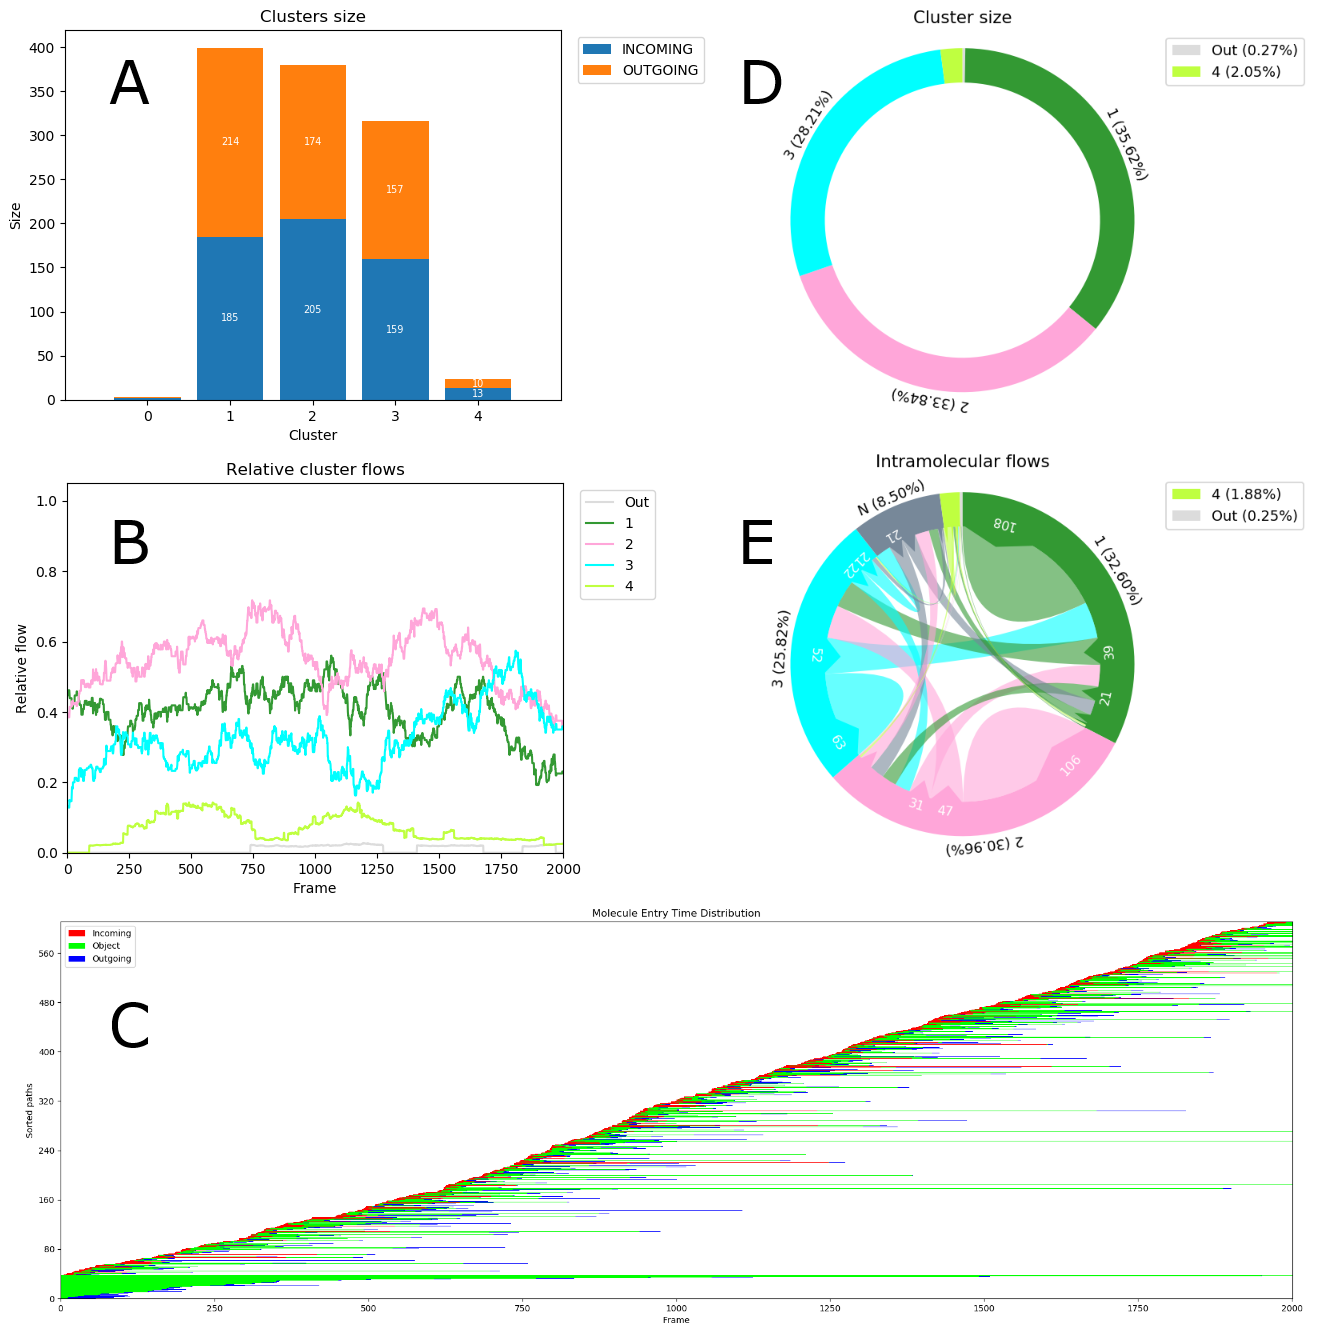
\includegraphics[width=\textwidth]{Tut3.1.png}
\caption{Results of \textit{kraken}: A) \textbf{Clusters size: barplot}. The barplots present the size of clusters (y axis) of each cluster (x axis) as a number of inlets (white digits on the barplots). Barplots are additionally divided to INCOMING (blue) and OUTGOING (orange), which mark number of traced molecules found within respective cluster that were entering or exiting the \textit{Scope}. B) \textbf{Relative clusters flows}. The plot indicates the relative flow of solvent molecules in clusters (y axis) in each frame of the simulation (x axis) in reference to the total flow in a given frame. C) \textbf{Molecule Entry Time Distribution}. The plot presents the colour-coded paths sorted by the moment they have entered the \textit{Scope} (axis y) in each frame of the simulation (axis x). Red indicate incoming paths, green inside the \textit{Object}, blue outgoing. D) \textbf{Cluster size: pie chart}. The pie chart shows the percentage value of the size (in number of inlets) of each cluster. E) \textbf{Intramolecular flows}. The pie chart presents the percentage value of the flow (in number of inlets) of  each cluster. The chart is enriched with information about direction and size of the flow (in number of inlets). \texttt{N} is not a cluster but indicates paths that have their beginning or end within the \emph{Scope}.}
\label{Tut3.1}
\end{figure*}

The \textbf{Relative clusters flows} shows the contribution of particular exits in total flow of the ligands in time ({Figure \ref{Tut3.1}B}).

The \textbf{Molecule Entry Time Distribution} plot presents the colour-coded paths sorted by the moment they have entered the \textit{Scope}. There are few water molecules that have entered the \textit{Scope}, went to the \textit{Object} and stayed there till the end of the simulation, they are mostly green. But some water molecules have problems with entering the \textit{Scope} (mostly red lines) and some other had difficulty exiting (mostly blue lines) (Figure \ref{Tut3.1}C). The user can easily find individual molecules by searching the \texttt{List of separate paths and properties} table in the \texttt{5\_analysis\_results.txt} file.

The \textbf{Cluster size} and \textbf{Intramolecular flows} graphs provide the information about the global molecules flow during the simulation. \textbf{Cluster size: pie chart} gives the information on the percentage value of the size of each cluster (Figure \ref{Tut3.1}D). The \textbf{Intramolecular flows} graph provides intuitive information on how much water molecules and in what direction have been exchanged between clusters (Figure \ref{Tut3.1}E). 

During the AQUA-DUCT analysis of the sample data, three almost equally big clusters were identified, namely \texttt{cluster\_1}, \texttt{cluster\_2}, and \texttt{cluster\_3}. The side cluster \texttt{cluster\_4} comprises of 1.88\% of all identified inlets \ref{Tut3.1}D. On the \textbf{Intramolecular flows} graph, one can easily observe the direction of the flow along with its size. Tracked molecules can enter and leave protein by the same or different entrance, e.g., the first main inlets cluster, \texttt{cluster\_1}, exchanges water molecules within itself, but also with \texttt{cluster\_2}, \texttt{cluster\_3} and \texttt{N}. It is shown that the flow can be also two-way (e.g. there is flow from \texttt{cluster\_1} to \texttt{cluster\_2} and from \texttt{cluster\_2} to \texttt{cluster\_1}) (Figure \ref{Tut3.1}E). 

On the \textbf{Intramolecular flows} graph, one can also observe a cluster named \texttt{N}. Technically, \texttt{N} is not a cluster but indicates paths that have their beginning or end within the \emph{Scope}. The size of the \texttt{N} "cluster" depends on size of the system and the length of the MD simulations. For longer simulations the relative size of the \texttt{N} "cluster" should decrease.

The \textbf{Scope and Object area and volume} plots present results based on the \texttt{ConvexHull} approximation. The plots of \textbf{Object area} and \textbf{Object volume} should be stable or otherwise there might be something wrong with the calculations. The shifts on the \textbf{Scope area} and \textbf{Scope volume} plots could indicate some information about the conformational changes of the protein structure (Figure \ref{Tut3.2}).

\begin{figure}[htb!]
\centering
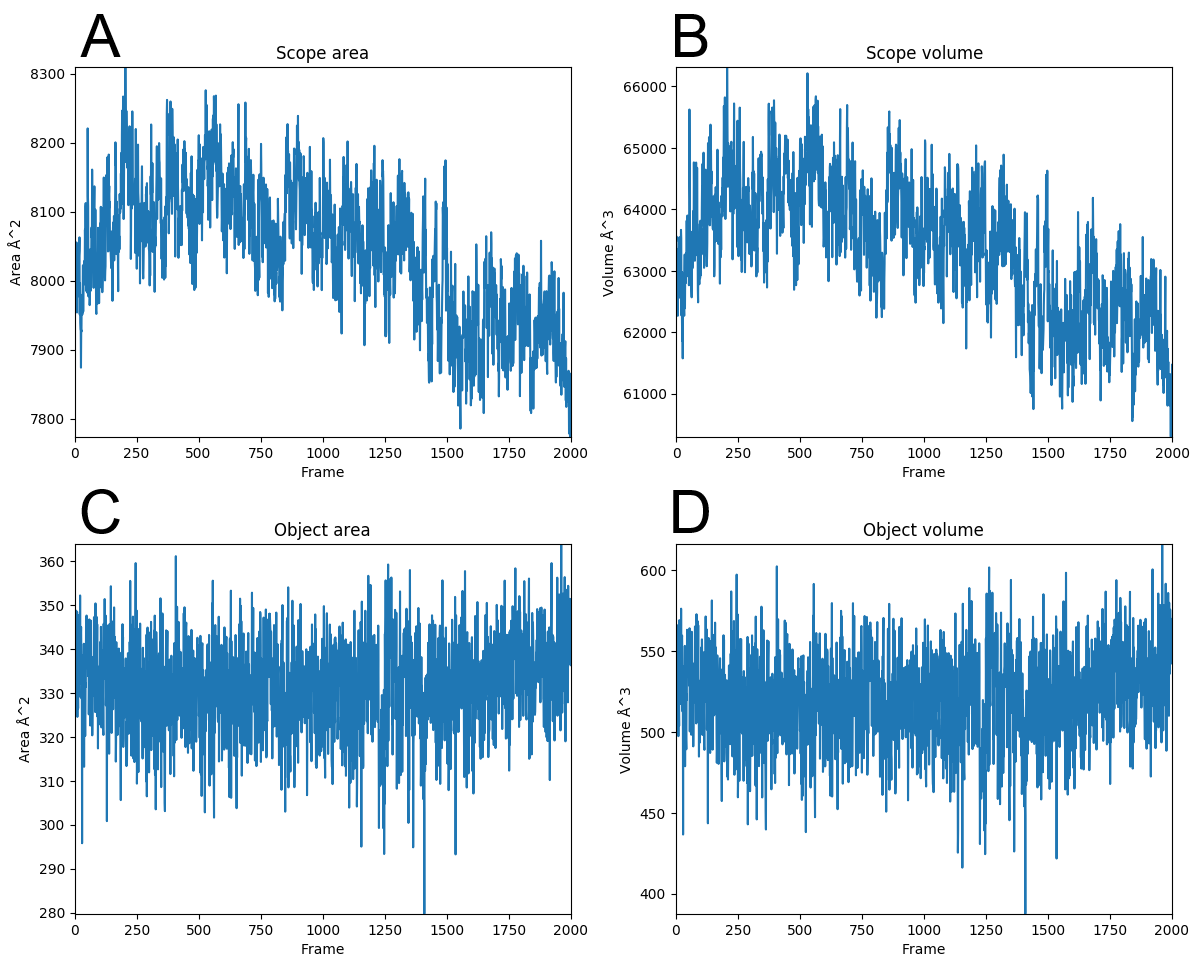
\includegraphics[width=0.5\textwidth]{Tut3.2.png}
\caption{Results of \textit{kraken}: A) \textbf{\textit{Scope} area}, B) \textbf{\textit{Scope} volume}, C) \textbf{\textit{Object} area} and D) \textbf{\textit{Object} volume}. The plots show the changes in \textit{Scope} and \textit{Object} size (axis y) in each frame of the simulation (axis x). Area is presented in in [Å\( \displaystyle ^{2}\)] and volume is presented in in [Å\( \displaystyle ^{3}\)]} 
\label{Tut3.2}
\end{figure}

The \textbf{Clusters area} plots are based on the inlets clusters density. The plot shows the area of each region of defined density for each cluster (Figure \ref{Tut3.3}).

\begin{figure}[htb!]
\centering
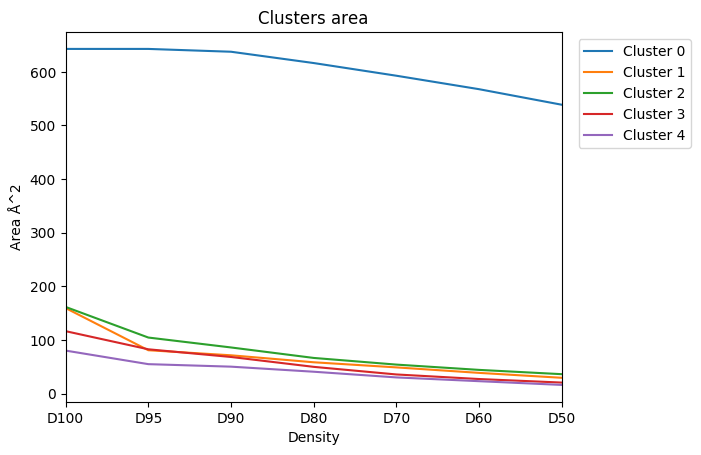
\includegraphics[width=0.5\textwidth]{Tut3.3.png}
\caption{Results of \textit{kraken}: \textbf{Clusters area}. The plot shows area (axis y) in [Å\( \displaystyle ^{2}\)] of every Cluster area isoline (axis x).}
\label{Tut3.3}
\end{figure}

In summary, the Tutorial 3 provides the user with statistical analysis of the sample data in accordance with the results visualized in the previous tutorial. In Tutorial 2, the user learned that AQUA-DUCT calculations provided information about the three main clusters, one side cluster and outliers cluster. The statistical data from Tutorial 3 additionally enriched the analysis with information about solvent flow between respective clusters, changes in \textit{Scope} and \textit{Object} areas and volumes, as well as distribution of molecules entry times. All this data is calculated by \textit{kraken} based on AQUA-DUCT result files, \texttt{5\_analysis\_results.txt} and \texttt{5\_analysis\_results.txt.csv}, which contain detailed information about the time of each molecule's entry/exit to/from \textit{Scope} and \textit{Object}. Data in these files is stored as tables, which can themselves be used to read information about the results, which provides the user a possibility to investigate the particulars of solvent flow throughout the course of the simulation along with rare events. 

Tutorial 3 presents the rest of the results that can be acquired through AQUA-DUCT calculations with \textit{valve}. In the next tutorials, the user will learn what kind of data can be calculated with \textit{pond}.

\subsection{Tutorial 4: Local distribution approach: hot-spots identification and energy profiles}

This tutorial shows how to perform solvent distribution analysis and calculate pockets, hot-spots, and energy profiles. Such analysis can be used to perform a rational protein re-design. Hot-spots can indicate residues that are attracting some molecular probes of particular physico-chemical properties (i.e. in the case of water molecules used as such a probe they can mark residues that create strong hydrogen bonds), or trap molecules due to gating movements. On the other hand, information on the energy barrier along a particular tunnel (here represented by a smooth path) can be used to identify amino acids that are creating obstacles during the small molecules transportation. The modification of such identified amino acids can lower the energy barrier and therefore speed up the flow of small molecules.

For this tutorial the user should use \href{http://www.aquaduct.pl/user-guide/}{sample data \#2} which comprises of topology and trajectory files of human soluble epoxide hydrolase in a water box and an additional \texttt{frames} directory which is used for time-window mode analysis described in the next tutorial. It is necessary for the calculations presented in this tutorial that the user provides \textit{pond} module with dump files (i.e., \texttt{2\_raw\_paths\_data.dump} and \texttt{3\_separate\_paths\_data.dump}) obtained as it was presented in Tutorial 1, as well as the trajectory, topology and configuration files downloaded from the AQUA-DUCT website.

The first part of this tutorial will focus on hot-spots analysis and the second part will focus energy profile calculations. Those calculations can be run collectively, but for the clarity, they will be run separately here.

The user should change their working directory to \texttt{2\_advanced\_analysis}, since for the purposes of this tutorial, one needs to use a different set of MD simulations data - sample data \#2. Prior to the advanced calculations, the user needs to create their own configuration file from the existing template:
\begin{lstlisting}
valve_run --dump-template-config > config.txt
\end{lstlisting}

Within the configuration file, the user needs to provide the names of trajectory and topology files from the sample data set \#2, along with the name of cache directory (here named \texttt{cache}), in which AQUA-DUCT will store the necessary data from each run of the calculations. The \emph{Scope} should be set to \texttt{protein} and the \emph{Object} definition is as follows: \texttt{(resname WAT) and (sphzone 5.0 (resid 98 or resid 146 or resid 259 or resid 229 or resid 287))}. The \texttt{add\_passing} option should also be used. For hot-spots calculations AQUA-DUCT uses local solvent distribution approach, therefore the hot-spots are determined as the most dense regions within the analysed macromolecule. \textit{Pond} can use two types of paths for the hot-spots calculations: i) only those molecules that entered both the \textit{Scope} and the \textit{Object}, and ii) all traced molecules that entered the \textit{Scope} (i.e., both \textit{passing paths} and standard paths). The second type of paths is called the passing paths. To use the information about the distribution of the solvent from the passing paths, the use of the \texttt{add\_passing} option is required.
\begin{lstlisting}[columns=fullflexible]
[global]
top = topology_hsEH_WAT.prmtop
trj = trajectory_hsEH_WAT.nc
cache_dir = cache

[traceable_residues]
scope = protein
scope_convexhull = True
object = (resname WAT) and (sphzone 5.0 (resid 98 or resid 146 or resid 259 or resid 229 or resid 287))
add_passing = resname WAT
\end{lstlisting}
The \texttt{add\_passing} option could be set to any molecular entity, such as water molecules, ions, ligands or co-solvents, which will be traced at the moment it enters the \emph{Scope}, even without entering the \emph{Object}. Therefore, while using this option, the user should keep in mind that such computations could be more time- and resource-demanding.

Clustering and visualization steps are not crucial and do not affect the results of calculations described in this tutorial, although running proper clustering and visualizing all available pathways that were used for the presented calculations could be useful. That is why the configuration file should also be adjusted. \texttt{auto\_barber} option should be set to \texttt{protein} in both \texttt{[separate\_paths]} and \texttt{[clustering]} sections to ensure the proper level of trimming paths. In the \texttt{[inlets\_clustering]} section the \texttt{create\_master\_paths} should be set to \texttt{True}, since the user would like to compare their raw and smooth paths with the master paths in further steps of this analysis. The following options in the \texttt{[visualize]} section should be set to \texttt{True}: \texttt{retain\_all\_types}, \texttt{all\_paths\_raw}, \texttt{all\_paths\_smooth}, \texttt{all\_paths\_split}, \texttt{paths\_raw}, \texttt{paths\_smooth}, \texttt{paths\_states}, \texttt{ctypes\_raw}, \texttt{ctypes\_smooth},  and \texttt{inlets\_clusters}. While most of the options are self-explanatory, three options should be explained: if the \texttt{all\_paths\_split} is set to \texttt{True} PyMOL will split the objects produced by \texttt{all\_paths\_raw} and \texttt{all\_paths\_smooth} into IN (red), OUT (blue), and OBJ (green and yellow) parts of paths; \texttt{paths\_states} will enable the visualization of all raw and smooth paths as separate states in PyMOL, and \texttt{retain\_all\_types} will enable the visualization of all paths. The \texttt{show\_molecule} and \texttt{show\_scope\_chull} options should be set to \texttt{protein} to enable the visualization of the analysed macromolecule, and the \texttt{show\_object\_chull} should be set to \texttt{(resname *) and (sphzone 5.0 (resid 98 or resid 146 or resid 259 or resid 229 or resid 287))}. The user should mind the small change in the definition of the \textit{Object} here, where the type of traced molecules was replaced by and asterisk (*) to ensure proper visualization of the \textit{Object} region.

\begin{lstlisting}
[separate_paths]
auto_barber = protein

[inlets_clustering]
create_master_paths = True

[visualize]
retain_all_types = True
all_paths_raw = True
all_paths_smooth = True
all_paths_split = True
paths_raw = True
paths_smooth = True
paths_states = True
ctypes_raw = True
ctypes_smooth = True
inlets_clusters = True
show_molecule = protein
show_scope_chull = protein
show_object_chull = (resname *) and (sphzone 5.0 (resid 98 or resid 146 or resid 259 or resid 229 or resid 287))

[clustering]
method = barber
auto_barber = protein
\end{lstlisting}

The prepared configuration file should be then used to run basic calculations with AQUA-DUCT (Figure \ref{Tut4.1}):
\begin{lstlisting}
valve_run -c config.txt --debug-file aq.log
\end{lstlisting}
On an Intel Core i7-4790 CPU @ 3.60 GHz machine these calculations take approx. 7 minutes. 
The user can now visualize the results in PyMOL and save the session (see Tutorials 1 and 2 for more details how to prepare the session containing objects of most interest):
\begin{lstlisting}
python 6_visualize_results.py --save-session session.pse
\end{lstlisting}

\begin{figure}[ht!]
\centering
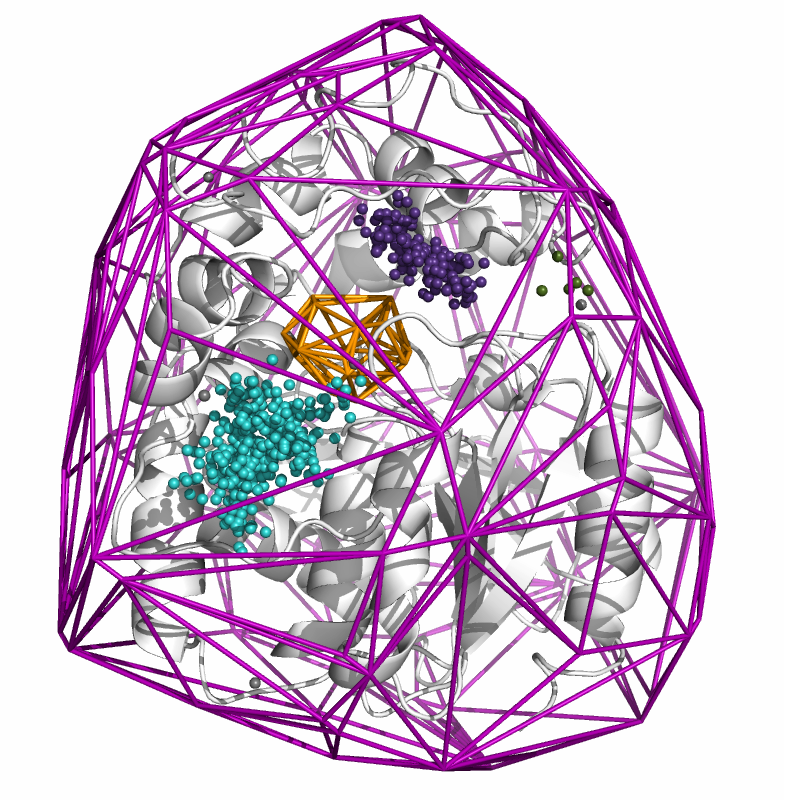
\includegraphics[width=0.5\textwidth]{Tut4.1.png}
\caption{Results of AQUA-DUCT calculations and clustering using sample data \#2. The \emph{Scope} is shown as purple shape, the \emph{Object} as orange shape and clusters are shown as coloured spheres.}
\label{Tut4.1}
\end{figure}

AQUA-DUCT uses module called \textit{pond} to handle the hot-spots and energy profile calculations. \textit{Pond} can be run directly in the command line. The user can type in the command below to see the help information:
\begin{lstlisting}
pond_run -h
\end{lstlisting}
Prior to hot-spots analysis, \emph{pond} needs to calculate pockets. Pockets represent the space of a particular macromolecule which was visited by tracked molecules during the simulation time. There are two types of pockets: Inner pocket represents places that were very often visited, while the Outer pocket stands for all the regions that were  penetrated. The user can modify the description of the Inner pocket by setting the \texttt{-{}-io-threshold} to a particular percentage value. By default, the median density value is used.

\begin{figure}[ht!]
\centering
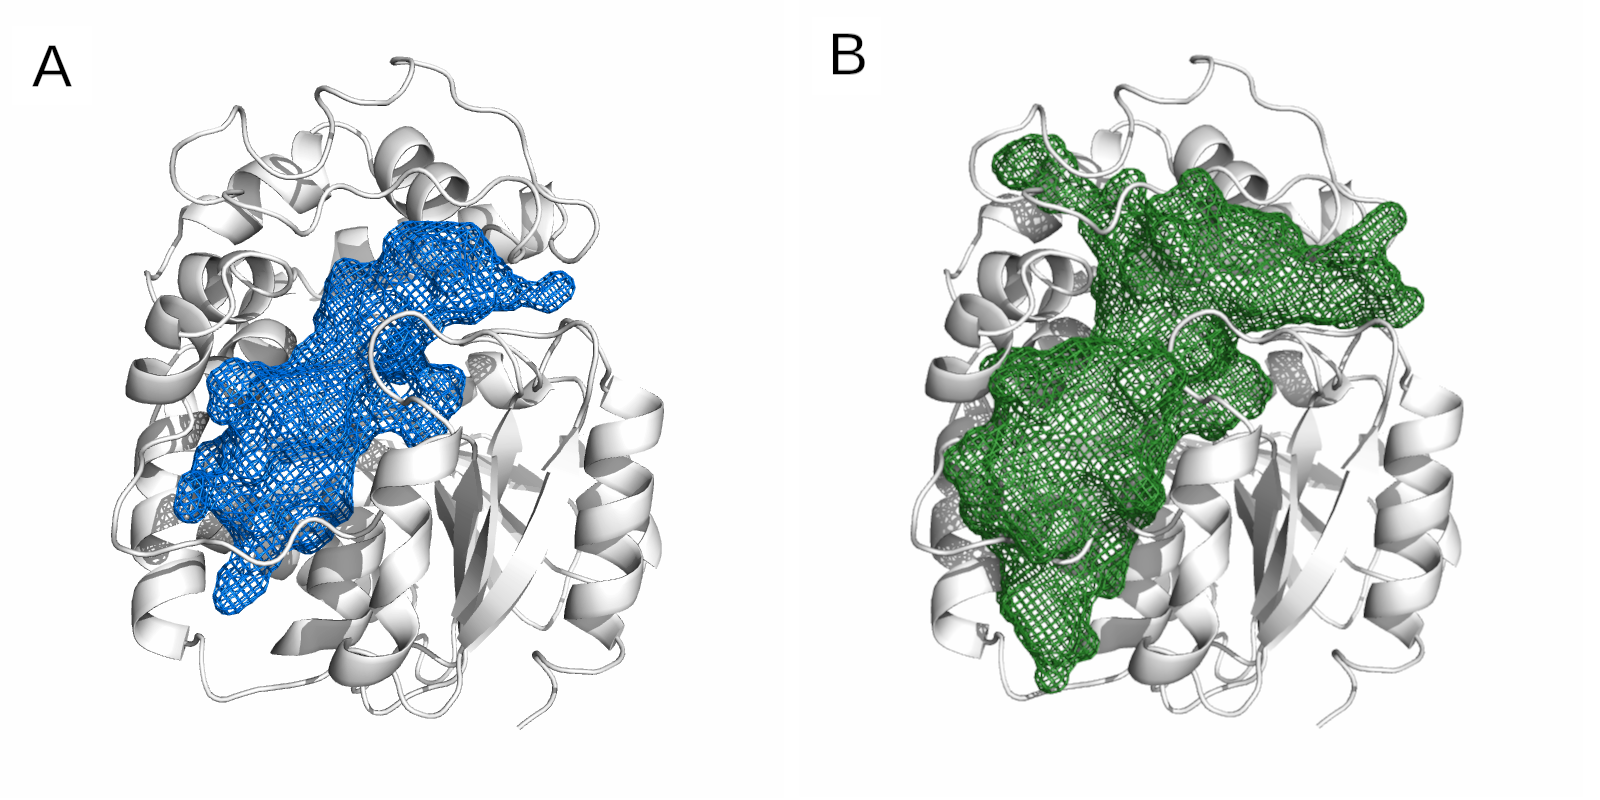
\includegraphics[width=0.5\textwidth]{Tut4.2.png}
\caption{Comparison of pockets calculated by \textit{pond}: A) Inner (in PyMOL marked as \texttt{inner\_full\_WAT\_local.mol2}) and B) Outer pocket (in PyMOL marked as \texttt{outer\_full\_WAT\_local.mol2}). The protein is shown as cartoon, Inner pocket is blue mesh and Outer pocket is green mesh.}
\label{Tut4.2}
\end{figure}

Hot-spots can be calculated in two ways: i) using the density information coming only from those paths that have visited the \emph{Object}, the so-called local hot-spots, and ii) including the more abundant density information coming from all the paths that have visited the \emph{Scope}, the so-called global hot-spots. For the global hot-spots calculation, the user should include the \texttt{add\_passing} option in the configuration file and also \texttt{-{}-raw} option provided in \emph{pond}. The user should also keep in mind that calculations of the global hot-spots are more demanding than the same calculations of local hot-spots.

To calculate the local hot-spots the user needs to run their calculations within a directory in which they saved the \texttt{3\_separate\_paths\_data.dump} file, along with the configuration file prepared for previous \emph{valve} run and using \emph{pond}. On an Intel Core i7-4790 CPU @ 3.60 GHz machine these calculations take 30 seconds.
\begin{lstlisting}
pond_run -c config.txt --debug-file pond_local.log --pockets --hotspots --reference-calc -r Hotspots_local/ --reference-mol 'resname WAT' --paths-types 'WAT' --output-suffix 'local'
\end{lstlisting}
The resulting data will be stored in Hotspots\_local directory. For hot-spots calculations, \emph{pond} also requires a reference density in bulk solvent (by default, the density of tracked water molecules - marked as WAT in the topology file; if in the user's topology file water molecules are marked differently, then they need to set the proper name using \texttt{-{}-reference-mol} option) to determine the density of identified hot-spots. Therefore, the \texttt{-{}-reference-calc} option is required. The reference value could be also provided by the user with the \texttt{-{}-reference-value} option and a particular density value should be entered in [kJ/mol/K].
\emph{Pond} will also store the results in user-defined directory, here in \texttt{Hotspots\_local} directory, determined using the \texttt{-r} flag. The \texttt{-{}-reference-mol} option allows determining for which type of molecules the reference density will be calculated, here only water molecules. The \texttt{-{}-paths-types} option limits calculations to given paths types, here also water molecules. Finally, the \texttt{-{}-output-suffix} option adds an appropriate suffix to the output files, so the user can identify the type of data for which the calculations were performed. 

In the command line the user should see the following information:
\begin{lstlisting}[columns=fullflexible]
Reference number of molecules: 3710 [molecules].
Reference density: 0.0554 [molecules/A^3].
Reference value: 7.2185 [kJ/mol/K].
\end{lstlisting}

\begin{Checklists}
\begin{checklist}{TIP}
\textbf{Reference value calculation in \textit{pond}}

In the case when the user would like to perform several pockets, hot-spots or energy profiles calculations using the same system, instead of using the \texttt{-{}-reference-calc} option and calculating the reference value each time anew, they can use \texttt{-{}-reference-value} option and type in the \textit{Reference value} calculated during the first run of \textit{pond} calculations.
\end{checklist}
\end{Checklists}

For computation of the global hot-spots (on an Intel Core i7-4790 CPU @ 3.60 GHz machine these calculations take approx. 3 minutes and 30 seconds), the user should use the command below:
\begin{lstlisting}[columns=fullflexible]
pond_run -c config.txt --debug-file pond_global.log --pockets --hotspots --raw --reference-value 7.2185 -r Hotspots_global/ --reference-mol 'resname WAT' --paths-types 'WAT' --output-suffix 'global'
\end{lstlisting}
\emph{Pond} will then calculate the global hot-spots using the information on the trajectory and topology files listed in the configuration file, as well as data stored in \texttt{2\_raw\_paths\_data.dump}. 
\emph{Pond} is also capable of dividing the provided simulation into smaller pieces, the so-called windows. The time-window analysis mode will be showed in detail in the next Tutorial.

Hot-spots and pockets are stored as \texttt{.mol2} files (herein as: \texttt{inner\_full\_WAT\_local.mol2}, \texttt{outer\_full\_WAT\_local.mol2}, \texttt{hotspots\_full\_WAT\_local.mol2}, \newline \texttt{inner\_full\_WAT\_global.mol2}, \texttt{outer\_full\_WAT\_global.mol2}, and \texttt{hotspots\_full\_WAT\_global.mol2},) which are easy to open using PyMOL. The user can open those files in their previously created AQUA-DUCT results PyMOL session. During pockets calculation \emph{pond} creates also a \texttt{volumes\_WAT\_local.dat} and \texttt{volumes\_WAT\_global.dat} in which the information about the Inner and Outer pockets' volumes are saved in [Å\( \displaystyle ^{3}\)]. AQUA-DUCT package consists of a Python script dedicated to hot-spots analysis which can be used in PyMOL to manipulate with the hot-spots representation. 

During the hot-spots calculations, \emph{pond} creates a \texttt{pond\_meta\_WAT\_local.json} file in which it stores the information of the reference density value. Using such information makes it possible for the user to manipulate the size of the obtained hot-spots and resize them according their density values (i.e., the most dense hot-spots will be bigger than those with lower density). PyMOL also offers an option to colour the hot-spots according to their density.

To use the \texttt{hs\_resize.py} script from the AQUA-DUCT package, the user should type in within the PyMOL console:
\begin{lstlisting}[columns=fullflexible]
run /path/to/hs_resize.py
hs_resize /path/to/pond_meta_WAT_local.json, hotspots_full_WAT_local
hs_resize /path/to/pond_meta_WAT_global.json, hotspots_full_WAT_global
\end{lstlisting}
where \texttt{path/to/hs\_resize.py} should be replaced by the exact path to the script and \texttt{path/to/pond\_meta\_WAT\_local.json} and \texttt{path/to/pond\_meta\_WAT\_global.json} by the exact path to the \texttt{.json} file. 

Please also note that the \texttt{hs\_resize.py} script uses two variables: the \texttt{.json} file and the name of the selection it should be used on (here it is \texttt{hotspots\_full\_WAT\_global}), but for local hot-spots it should be set as \texttt{hotspots\_full\_WAT\_local}.
The path to the script could be easily found by typing:
\begin{lstlisting}
which hs_resize.py
\end{lstlisting}
in the command line.

To additionally colour the hot-spots according to their density values, the user should type in the PyMOL console:
\begin{lstlisting}[columns=fullflexible]
spectrum pc, blue_white_red, hotspots_full_WAT_local
spectrum pc, blue_white_red, hotspots_full_WAT_global
\end{lstlisting}

\begin{figure}[ht!]
\centering
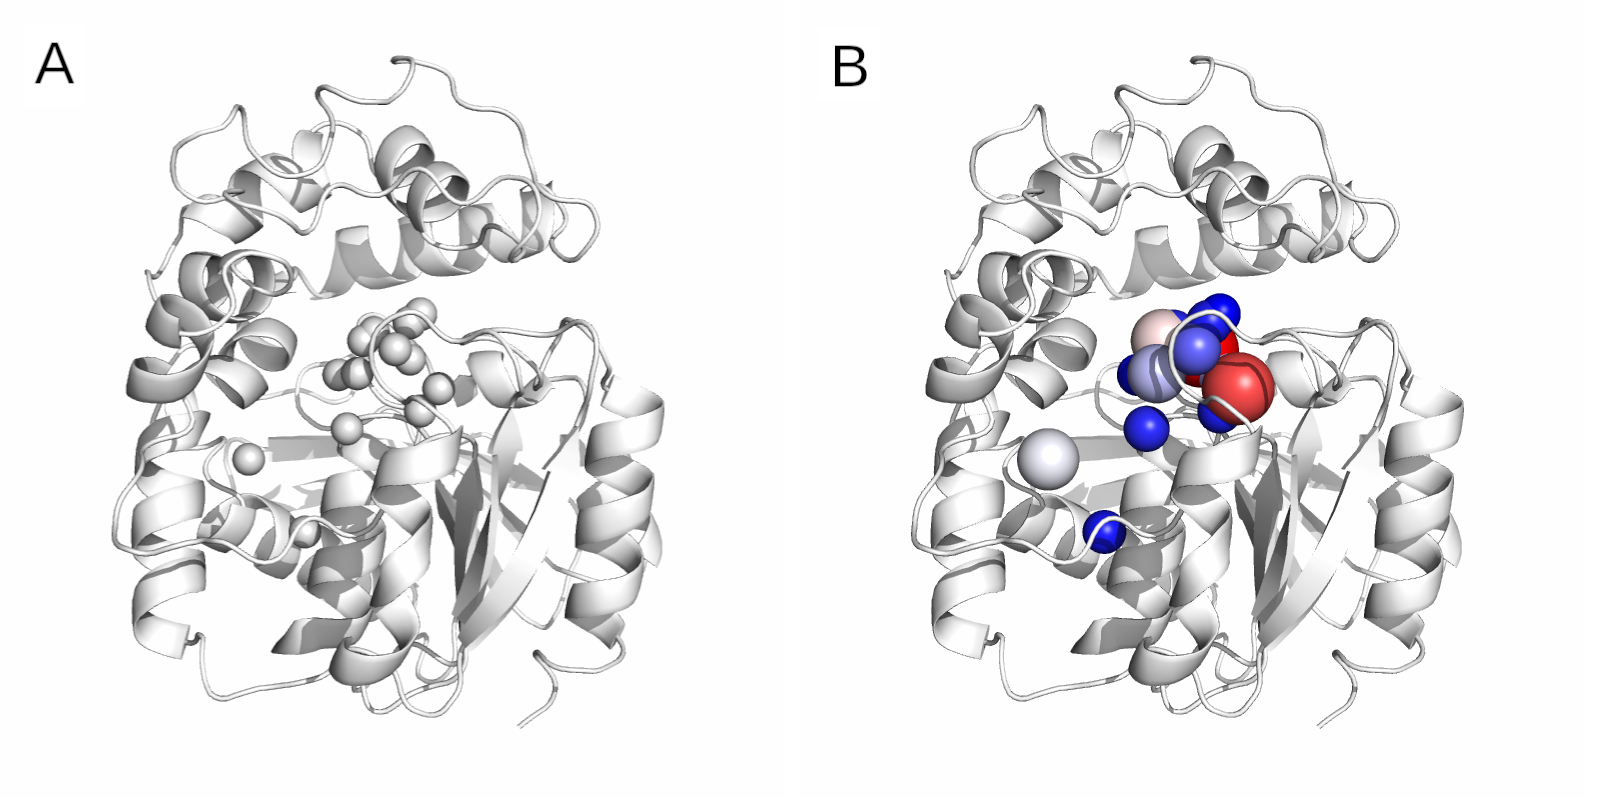
\includegraphics[width=0.5\textwidth]{Tut4.3.png}
\caption{Local hot-spots calculated by \textit{pond}: A) before resizing and B) after resizing. The protein is shown as cartoon, the hot-spots on the left panel are shown as spheres, and hot-spots on the right panel are resized and colour-coded according to their density values. The hot-spots are marked in PyMOL as \texttt{hotspots\_full\_WAT\_local}.}
\label{Tut4.3}
\end{figure}

Please note that PyMOL offers many different colour palettes and that the last option denotes the name of the hot-spots object in a PyMOL session. Most local hot-spots are located in the vicinity of the active site cavity, and within the \emph{Object}. Two of them are located below the active site, within the core domain of the human soluble epoxide hydrolase structure. The local hot-spots overlap with the \texttt{inner\_full\_WAT\_local} pocket. The \texttt{outer\_full\_WAT\_local} pocket represents the protein's interior which is accessible for the tracked molecules during the course of molecular dynamics simulations. When compared with the local hot-spots, global hot-spots were identified within the interior of the protein's core domain, three hot-spots were found inside the interior of the cap domain. Two more hot-spots were identified at the border between the core and the cap domain. The location of the global hot-spots near the entrances/exits to the active site suggests that modification of residues adjacent to the entrance/exits may modify small molecules accessibility to the active site. The \texttt{inner\_full\_WAT\_global} pocket represent the protein's interior as well as some cavities located on the protein surface. Most of the global hot-spots are located within small cavities of the \texttt{inner\_full\_WAT\_global} pocket. The \texttt{outer\_full\_WAT\_global} covers the maximum accessible volume of the protein's interior and its surface.

\begin{figure}[ht!]
\centering
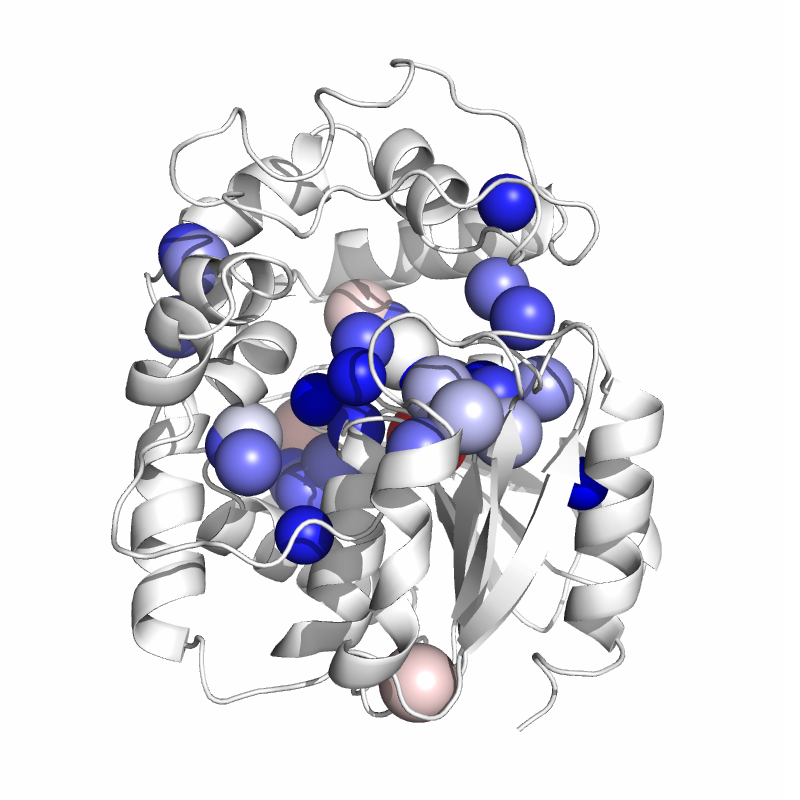
\includegraphics[width=0.5\textwidth]{Tut4.4.png}
\caption{Global hot-spots calculated by \textit{pond} after resizing. The protein is shown as cartoon, the hot-spots are resized and colour-coded according to their density values. The hot-spots are marked in PyMOL as \texttt{hotspots\_full\_WAT\_global}.}
\label{Tut4.4}
\end{figure}

Energy profile calculations are based on the density of traced molecules inside the \emph{Scope} and the Boltzmann distribution. Such calculations require a reference density value and a particular pathway along which the energy profile will be calculated. The selected path should be additionally smoothed so that it will represent the general overview of the particular passage. In the case where a raw path is used for the energy profile calculations, it will provide a very chaotic and knotted profile. For more information about smoothing paths the user is encouraged to see the \href{http://www.aquaduct.pl/smoothing-paths/}{Smoothing paths tutorial} on the AQUA-DUCT website.

The energy profile is calculated according to Boltzmann inversion. Similar method was used in \cite{Rao2017} paper. Following equation relates free energy with density of molecules:

\[ \textstyle n\left(z\right) = C \cdot \textstyle e^{ \textstyle \left(\frac{-E\left(z\right)}{kT}\right)} \]
where \textit{z} is point in the space, preferably along some kind of a path, \textit{n(z)} is density of molecules in point \textit{z}, \textit{C} is a normalization constant, \textit{E} is free energy, \textit{k} is Boltzmann’s constant, and \textit{T} is temperature.
One can easily transform the above equation to calculate energy:

\[ \displaystyle E\left(z\right) = -kT\ln\left( n\left( z\right)\right) - kT\ln\left(C\right) \]
Term \( \displaystyle kT\ln\left(C\right)\) does not depend on \textit{z} and can be determined by assumption that free energy in the bulk of traced molecules (solvent) is zero. Please also note that option \texttt{-{}-temperature} allows to set desired temperature in Kelvins.

Here the authors present a paths smoothing method to adjust the selected path so it will represent the shape of the tunnel along which molecules are able to flow (the user is also encouraged to compare this smoothed path with the overall master path -  \texttt{3\_2\_raw\_master}. Too intensive smoothing may provide biased results, for example in a situation when the path will pass through regions occupied by macromolecule's atoms and cause a bias in the results, as shown in Figure \ref{Tut4.5}. The user should ensure that any chosen path resembles the shape of the tunnel and does not stick out of the internal pocket.

For the presented sample data \#2, the user should consider adding the following smoothing options to their configuration file prior to running the energy profile calculations:
\begin{lstlisting}
[smooth]
method = window
recursive = 60
\end{lstlisting}
and set \texttt{execute} to \texttt{run} in the \texttt{[separate\_paths]} section of the configuration file. Setting \texttt{execute} to \texttt{run} and re-running AQUA-DUCT calculations enables AQUA-DUCT to load and read previously generated files from the two previous stages (i.e., \texttt{1\_traceable\_residues\_data.dump} and \texttt{2\_raw\_paths\_data.dump} files) and start calculations from the \texttt{[separate\_paths]} stage. More details on the \texttt{execute} option are provided in the Tutorial 2. 
\begin{lstlisting}
[separate_paths]
execute = run
\end{lstlisting}
The user can save the modified configuration file as \texttt{config\_smooth.txt}.

To keep all the data and avoid overwriting the files in next run of calculations, we recommend the user to copy the \texttt{3\_separate\_paths.dump}, \texttt{4\_inlets\_clustering\_data.dump}, \texttt{5\_analysis\_results.txt}, \texttt{5\_analysis\_results.txt.csv}, \texttt{6\_visualize\_results.py}, and \texttt{6\_visualize\_results.tar.gz} to the separate directory, called for example \texttt{run\_1}.

The user should now re-run AQUA-DUCT calculations:
\begin{lstlisting}
valve_run -c config_smooth.txt --debug-file aq_smooth.log
\end{lstlisting}

When the calculations finish and paths are smoothed (it take approx. 2 minutes and 30 seconds on an Intel Core i7-4790 CPU @ 3.60 GHz machine), the user can visualize the results:
\begin{lstlisting}
python 6_visualize_results.py --save-session session_smooth.pse
\end{lstlisting}
and compare the \texttt{smooth\_paths} in the PyMOL session with those from the previous session (\texttt{session.pse}). 

The user needs to select the path along which they want to calculate the energy profile. The \texttt{5\_analysis\_results.txt} file provides the user a list of all identified pathways along with more detailed information on the tracked molecules. The contents of this file were discussed previously in Tutorial 3. By default, the paths in \texttt{5\_analysis\_results.txt} file are listed according to the tracked molecule ID and loaded into the PyMOL session in the same order. For example: the path 12 in PyMOL session has the \textbf{Path ID} of 0:650:0, and path 109 has ID: 0:3972:0. The number of the path in the PyMOL session is equal to the first column (\emph{Nr}) in the \texttt{List of separate paths and properties} table. The \textit{Path ID} is in the second column (\emph{ID}). The user should keep in mind that they want to use the smooth path and should always use the \texttt{-{}-path-smooth} option.

To run the energy profile calculation along the smoothed path, the user should type:
\begin{lstlisting}
pond_run -c config.txt --debug-file pond_energy_1961.log --energy-profile --path-id 0:1961:0 --path-smooth --reference-value 7.2185 -r Energy_profile/ --reference-mol 'resname WAT' --paths-types 'WAT'
\end{lstlisting}
This calculations take approx. 55 minutes on an Intel Core i7-4790 CPU @ 3.60 GHz machine.
The user is encourage to calculate a similar energy profile along a different pathway (ID: 0:650:0) and compare the results.
\begin{lstlisting}
pond_run -c config.txt --debug-file pond_energy_650.log --energy-profile --path-id 0:650:0 --path-smooth --reference-value 7.2185 -r Energy_profile/ --reference-mol 'resname WAT' --paths-types 'WAT'
\end{lstlisting}
The calculations take approx. 60 minutes on an Intel Core i7-4790 CPU @ 3.60 GHz machine.

After the calculations, \emph{pond} will return two files, one with a graphical representation of the energy profile (here: \texttt{path0:1961:0\_\_radius.mol2} and \texttt{path0:650:0\_\_radius.mol2}) and the second with the results of energy calculations along the smoothed path (here: \texttt{path0:1961:0\_\_radius.dat} and \texttt{path0:1961:0\_\_radius.dat}). The user can open the \texttt{.mol2} file in their previously generated PyMOL session, while the \texttt{.dat} file can be easily used in their favourite plotting software to create a 2D plot of the energy profile (Figure \ref{Tut4.5}).

\begin{figure*}[ht!]
\centering
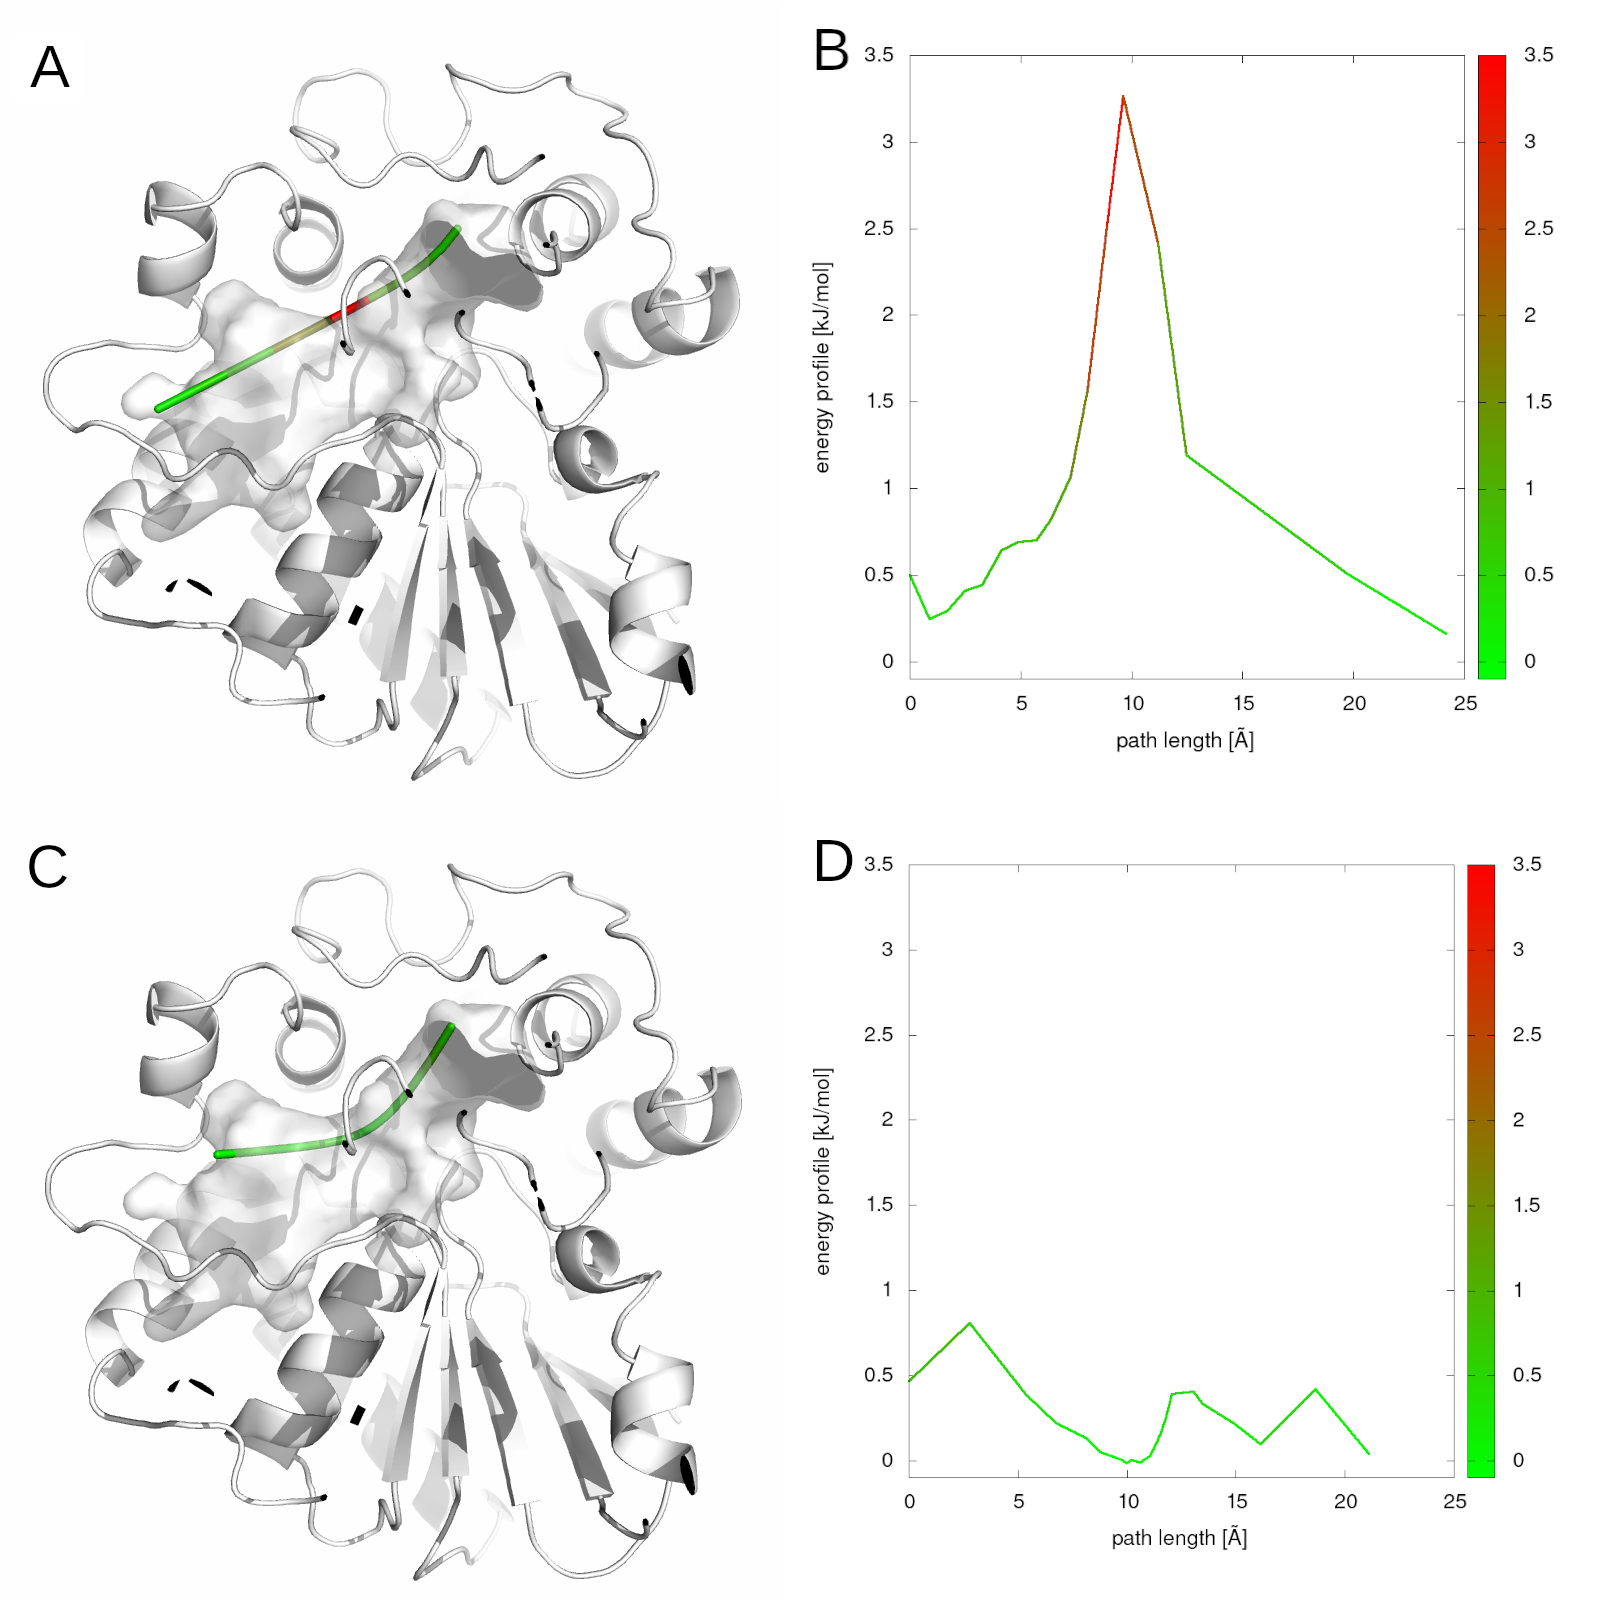
\includegraphics{Tut4.5.png}
\caption{Energy profile calculated along the paths number 12 (ID: 0:650:0) and 48 (ID: 0:1961:0). A) and C) Protein structure with visualized energy profile, B) and D) 2D plot of energy profile. The protein is shown as cartoon with \texttt{inner pocket} shown as transparent surface and the energy profile is shown as a line - the red parts of the profile indicate energy barriers, while green parts of the path represent regions without energy barriers. Energy profiles are marked in PyMOL as \texttt{path0:650:0\_\_radius} and \texttt{path0:1961:0\_\_radius}.}
\label{Tut4.5}
\end{figure*}

Once again, using the \texttt{spectrum} command in PyMOL, the user can colour the energy profile according to the energy values along the selected path by typing:
\begin{lstlisting}
spectrum pc, green_red, path0:650:0__radius
spectrum pc, green_red, path0:1961:0__radius
\end{lstlisting}
The green parts of the profile mark those regions of the protein interior in which no obstacles or energy barriers were found. The red part of the path indicate regions with energy barriers. 

In the case of the paths presented in this example, path 0:650:0 is too intensively smoothed, it sticks out of the inner pocket and in consequence shows a high energy barrier in the active site cavity (Figure \ref{Tut4.5} A, C). This example shows a potential error which the user should avoid. 
The second path 0:1961:0 resembles the shape of the analysed tunnel and its overall energy profile is low, which in the case of an epoxide hydrolase, an enzyme which utilizes water molecules for catalysis, represent a constant flow of water molecules through the active site (Figure \ref{Tut4.5} B, D).

\begin{Checklists}
\begin{checklist}{TIP}
\textbf{Choosing paths for energy profile calculation}

When searching for a path which can be used to calculate the energy profile along it, the user should ensure that the path represents the shape and geometry of the tunnel. The selected path needs to be smoothed, so that it does not contain any knots or twines and it cannot stick out from the internal cavities of the macromolecule.
\end{checklist}
\end{Checklists}

\subsection{Tutorial 5: Time-window analysis}

Both calculations presented in the previous Tutorials (i.e., pockets, hot-spots, and energy profiles) can be calculated for the whole simulation, but can also be performed on smaller pieces of trajectory, using the so-called windows. Such an analysis allows the user to compare the local and global pictures of the analysed features in different parts of the MD simulations and thus provide access to a description of different states, such as an open and closed conformation. By default, the entire trajectory is covered, so that is only one big window. Using the \texttt{-{}-wsize} option the user is able to manipulate the size of windows (in frames), and using the \texttt{-{}-windows} options the user is able to change the number of windows. Therefore, the windows can overlap with each other when those options are used.
To calculate the proper number of windows evenly spanning over the trajectory, the user can use the following equation:
 
\[ \displaystyle WINDOWS = \frac{TOTAL - WSIZE}{SHIFT} + 1 \]
where WINDOWS is a desired number of windows, TOTAL is total length of trajectory, and SHIFT is WSIZE - OVERLAP.

\begin{figure*}[ht!]
\centering
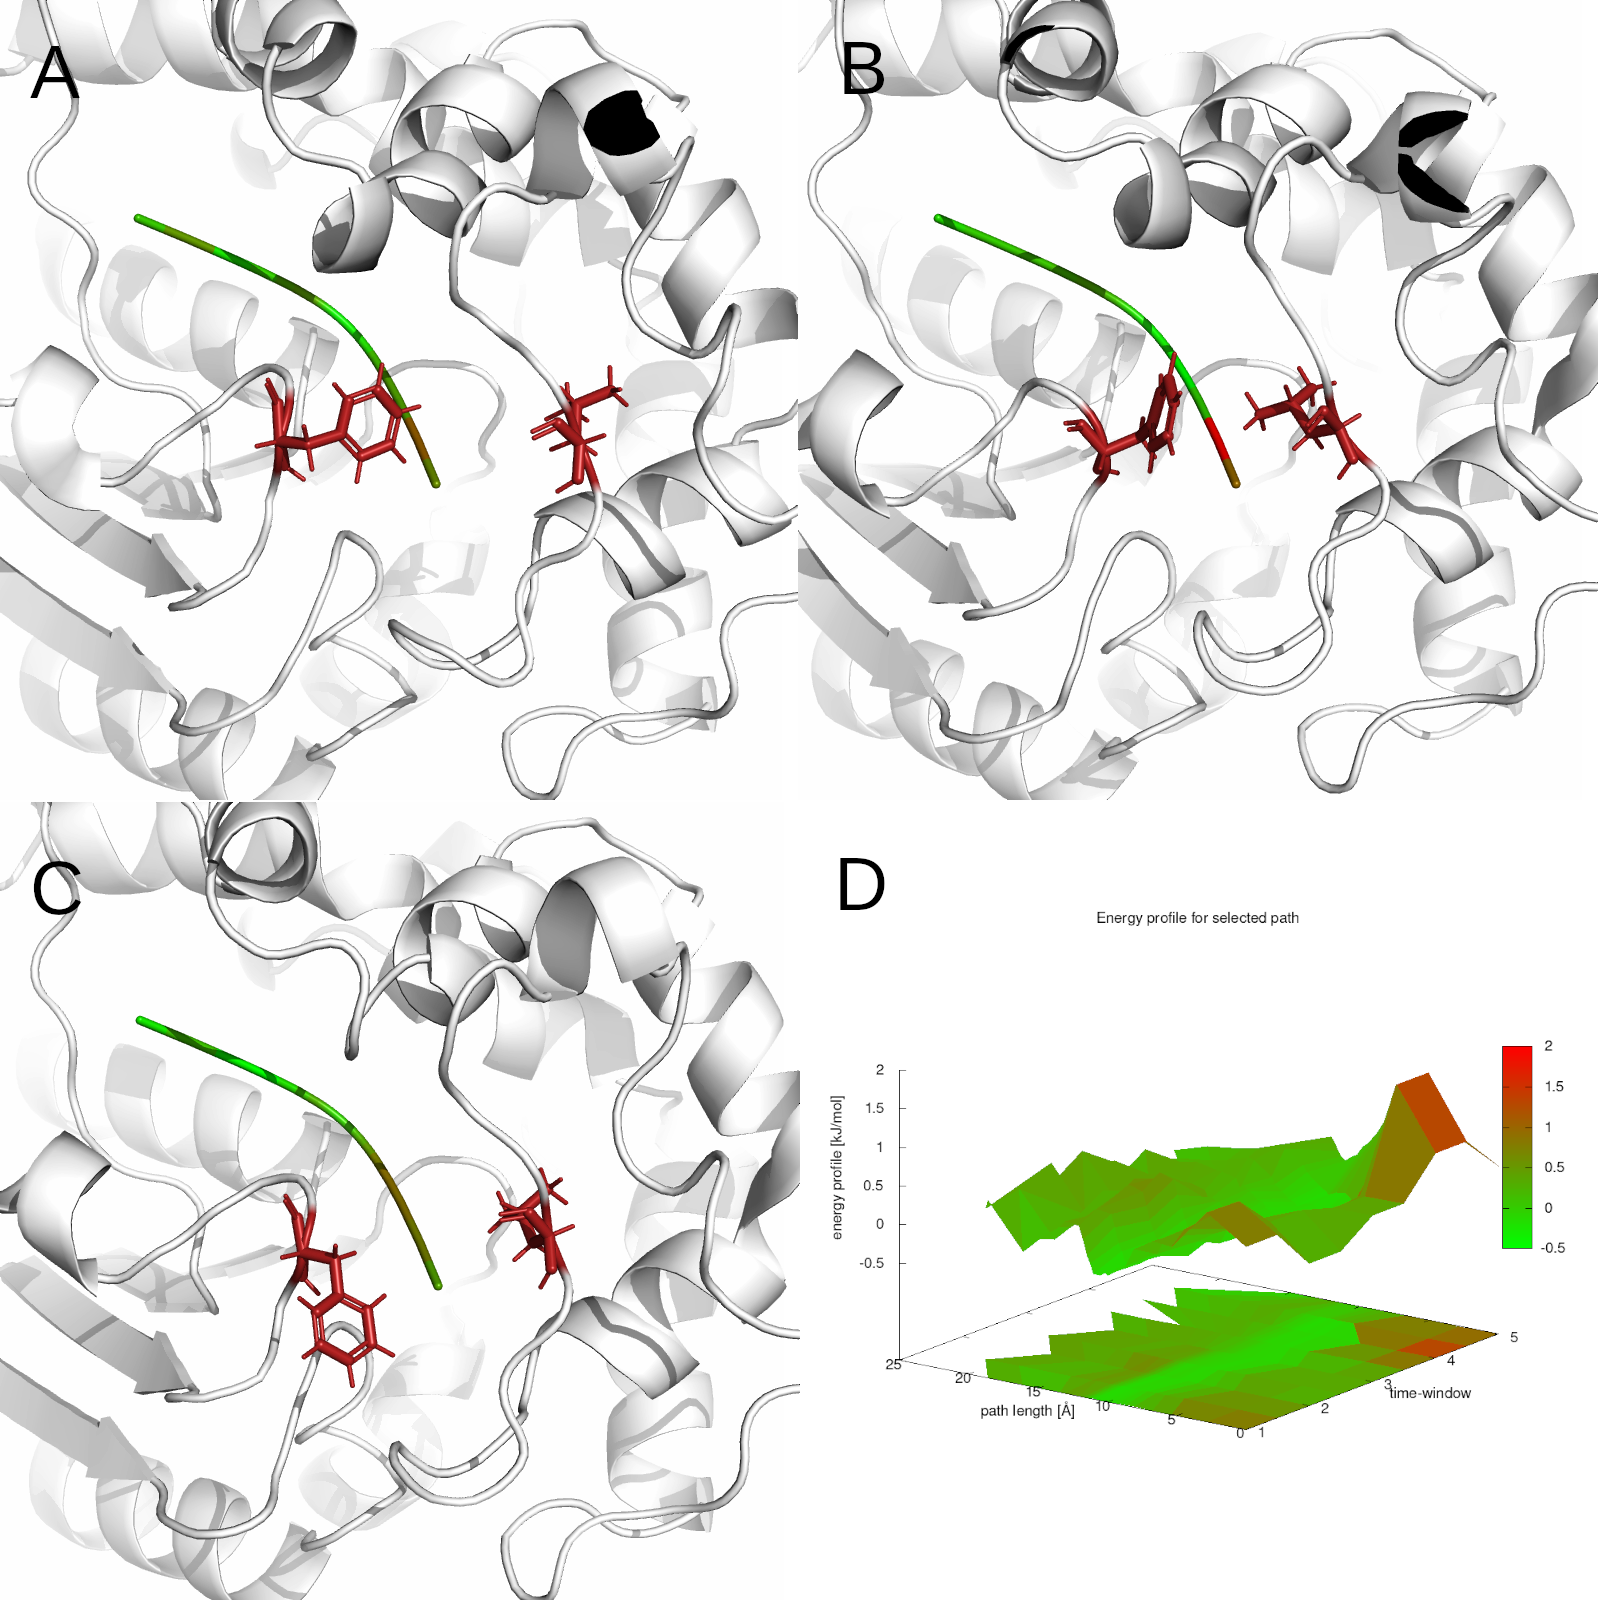
\includegraphics{Tut4.6.png}
\caption{The energy profile calculated along the path number 48 (Path ID: path0:1961:0) using the time-window mode of analysis. The starting point of the path is located between the cap and the core domains, and the access to the tunnel which the path represents is regulated by Leu180 and Phe260 (shown as red sticks). A) Frame 199; the entrance to the tunnel is wide open, the energy profile shows no obstacles. B) Frame 1399; the entrance to the tunnel is narrow, the energy profile shows obstacles at its beginning. C) Frame 1799; the entrance to the tunnel gets wider, so the energy profile shows smaller obstacles. D) The 3D plot of the energy profile along the selected path in 5 windows. The red parts of the profile represents energy barriers. The molecule presented in each panel is marked in PyMOL as \texttt{frame\_199}, \texttt{frame\_1399}, and \texttt{frame\_1799}, respectively and the Leu180 and Phe260 residues are shown as red sticks. The energy profile is shown as coloured line marked in PyMOL as \texttt{path0:1961:0\_\_WX\_WAT\_global}, and on each panel different state of the profile is shown: the first, the fourth, and the fifth, respectively.}
\label{Tut4.6}
\end{figure*}

Using time-window mode is recommended in cases where the macromolecule is rapidly changing its conformation what can affect the flow of tracked molecules. For the presentation of the time-window mode, the user should examine path number 48 (ID:~ 0:1961:0), to be able to observe the effect of conformational changes on the energy profile shape. They should also examine the time evolution of the global hot-spots. They are encouraged to run the local hot-spots calculations and compare the results (more information about calculating the local hot-spots are shown in the Tutorial 4).

The sample data \#2 consist of 2,000 frames (10 ns saved each 5 ps). For demonstration purposes, the simulation will be divided into 5 windows, 400 frames each, and the windows will not overlap. The calculations presented below take approx. 39 minutes on an Intel Core i7-4790 CPU @ 3.60 GHz machine.
To run such analysis the user should write in the command line:
\begin{lstlisting}
pond_run -c config.txt --debug-file pond_energy_wi5_1961.log --energy-profile --path-id 0:1961:0 --path-smooth --hotspots --pockets --windows 5 -- wsize 400 --raw --reference-value 7.2185 -r Analysis_in_windows/ --reference-mol 'resname WAT' --paths-types 'WAT' --output-suffix 'global'
\end{lstlisting}
The results will be stored in Analysis\_in\_windows directory.

Once again the user will be provided with the files consisting of results of pockets, hot-spots and energy profile analysis. In the case of generated \texttt{.mol2} files: pockets (\texttt{inner\_full\_WAT\_global.mol2}), (\texttt{outer\_full\_WAT\_global.mol2}), \hfill hot-spots (\texttt{hotspots\_full\_WAT\_global.mol2}), \hfill and \newline energy profile calculations \newline (\texttt{path0:1961:0\_\_WX\_radius\_WAT\_global.mol2}, their representations are possible to display in PyMOL as separate states corresponding to the consecutive windows. The numerical data from the energy profile calculations (i.e., the \texttt{.dat} files) the user will be provided with several different \texttt{.dat} files, each file corresponding to each of the calculated windows. The number of particular window for which the energy profile was calculated is marked in the file name, e.g., \texttt{path0:1961:0\_\_W1\_radius.dat} states for the first window, while \texttt{path0:1961:0\_\_W5\_radius.dat} for the fifth.

The \texttt{hs\_resize.py} script and the \texttt{spectrum} command will work for the data calculated in windows in the same way as it was presented previously in the Tutorial 4. From the energy profile data, the user is able to create a 3D plot (in their favourite plotting software) of the time evolution of the energy profile along the selected pathway .

For the purpose of this analysis the user needs to use three MD simulation snapshots located in the \texttt{frames} directory, namely \texttt{frame\_199.pdb}, \texttt{frame\_1399.pdb}, and \texttt{frame\_1799.pdb} files, and open them within the previously generated PyMOL session. The entrance point of the analysed path is located in the \texttt{cluster\_3} which is placed at the border between the cap and the core domains. The entrance is controlled by two residues, Leu180 and Phe260 (numbering according to the trajectory file). At the beginning of the simulation, as shown in the first frame (i.e., \texttt{molecule0}) and frame 199, the entrance is wide open, while in frame 1399 (i.e., in the middle of the fourth window), the entrance gets very narrow. In frame 1799 (i.e., in the middle of the fifth window) the entrance widens up. Figure \ref{Tut4.6} shows the time evolution of the entrance and the presence of an energy barrier at the beginning of the selected path. The global hot-spots analysis supports this observation; there are more hot-spots near the entrance to the \texttt{cluster\_3} in the fourth window than in other windows (data not shown on the figure). The time-window mode of analysis is helpful in the cases when the macromolecule is flexible and often changes its conformation, which can affect the solvent transportation. However, the user should keep in mind the fact, that the time-window mode of calculations is more time-consuming than a similar calculation ran for the whole simulation.
\pagebreak

\subsection{Tutorial 6: Multiple solvents analysis}

This tutorial shows how to analyse the system with more than one solvent. In such a case, each type of small molecule works as a different type of molecular probe and the results of calculations can be used e.g. as an approximation of the study of the passage of hydrophobic molecules or for pharmacophore description during the drug design process. Here, the main focus will be on obtaining the information about pockets and hot-spots for particular solvent using the \emph{pond} module. The user should bear in mind that any analyses that the user wants to perform using the \emph{pond} module requires prior calculations with the \emph{valve} module. This is because the \emph{pond} uses the information that are stored in the \texttt{2\_raw\_paths\_data.dump} and \texttt{3\_separate\_paths\_data.dump}, respectively. 

Herein, the user should use \href{http://www.aquaduct.pl/user-guide/}{sample data \#3} which comprises of topology and trajectory files of human soluble epoxide hydrolase inside a box containing water molecules in a mixture with acetonitrile molecules. Since the user will now use another set of sample data, sample data \#3, they should change their working directory to \texttt{3\_cosolvents\_analysis} in order to not override their previously generated results.

The user will use the knowledge acquired during performing Tutorial 1, 2, and Tutorial 4. To print and save the template configuration file, the user should use the following command in the command line:
\begin{lstlisting}[columns=fullflexible]
valve_run --dump-template-config > config.txt
\end{lstlisting}
The config.txt file will be created in the directory in which the command was launched. After opening the configuration file, the first modification that needs to be done is to enter the appropriate \texttt{[global]} settings. The proper path to both topology and trajectory files must be provided and setting a path to the directory for cache data is advised. 
\begin{lstlisting}
[global]
top = topology_hsEH_WAT_ACN.prmtop
trj = trajectory_hsEH_WAT_ACN.nc
cache_dir = cache
\end{lstlisting}
After making changes in the \texttt{[global]} section, proper modification in the \texttt{[traceable\_residues]} section needs to be done. The user has to enter the definition of both \emph{Scope} and \emph{Object}. Since the tracking of water and acetonitrile molecules should be performed inside the whole protein, the \textit{Scope} needs to be defined as \texttt{protein}. The \emph{Object} definition will be set as water and acetonitrile molecules (resname \textbf{WAT} or resname \textbf{ACN}) within 5 Å sphere of the centre of geometry defined by active site residues (residues 98, 146, 229, 259 and 287). Therefore, it should be defined as: \texttt{(resname WAT or resname ACN) and (sphzone 5.0 (resnum 98 or resnum 146 or resnum 229 or resnum 259 or resnum 287))}. The last change that the user should make in the \texttt{[traceable\_residues]} section is to modify the \texttt{add\_passing} option. This option allows to track molecules even if they did not visit the \emph{Object} during the simulation time. This is especially important in the subsequent \emph{pond} calculations for global hot-spots which are built on the basis of all paths that have visited the \emph{Scope}. To include both \textbf{WAT} and \textbf{ACN} paths, in the \texttt{add\_passing} option, type: \texttt{(resname WAT or resname ACN)}.
\begin{lstlisting}
[traceable_residues]
scope = protein
scope_convexhull = True
object = (resname WAT or resname ACN) and (sphzone 5.0 (resnum 98 or resnum 146 or resnum 229 or resnum 259 or resnum 287))
add_passing = (resname WAT or resname ACN)
\end{lstlisting}
In the section \texttt{[raw\_paths]}, there is no need to change any option, while in the \texttt{[separate\_paths]} section, the \texttt{auto\_barber} should be set to \texttt{protein} to properly trim the paths. The \texttt{auto\_barber} option should also be set to \texttt{protein} in the \texttt{[clustering]} section, where the default \texttt{auto\_barber} method will be used for clustering. 
\begin{lstlisting}
[separate_paths]
auto_barber = protein

[clustering]
method = barber
auto_barber = protein
\end{lstlisting}
As it was shown in the Tutorial 2, there is a possibility to create a cluster of outliers from other clusters with small number of inlets (e.g. clusters that contain only one inlet). To do so, the user should change the following options in the \texttt{[inlets\_clustering]} section: \texttt{detect\_outliers} to \texttt{True} and \texttt{singletons\_outliers} to \texttt{1}.  The user can also set the option \texttt{renumber\_clusters} to \texttt{True}, so that the numbering of the obtained clusters will correspond to their size.
\begin{lstlisting}
[inlets_clustering]
detect_outliers = True
singletons_outliers = 1
renumber_clusters = True
\end{lstlisting}
When the user will visualize results in PyMOL (Figure \ref{Tut6.1} and Figure \ref{Tut6.2}), there will be no need to add any additional clustering section nor divide/join clusters to improve the clustering. Moreover, if the user is only interested in hot-spots and/or pockets analyses, there is no need for special optimisation of clustering. 
In the section \texttt{[analysis]}, there is no need to change any option, since there is not necessity to calculate the size of the \emph{Scope} and \emph{Object}.
The last options, that the user should modify, are located in the \texttt{[visualize]} section. In this tutorial, the following options should be set to \texttt{True}: \texttt{split\_by\_type, retain\_all\_types, all\_paths\_raw, all\_paths\_smooth, all\_paths\_split, paths\_raw, paths\_smooth, paths\_states, ctypes\_raw, ctypes\_smooth, inlets\_clusters, cluster\_area}. Option \texttt{split\_by\_type} is very helpful during the visualization of the results in PyMOL, when there is more than one type of traced molecules in the system. This option splits all objects that correspond to particular types of traced molecules. Appropriate molecule name is added to the created objects. Option \texttt{show\_molecule} should be set to \texttt{protein}, since the user wants to visualize the analysed macromolecule. Option \texttt{show\_scope\_chull} should be set to \texttt{protein}, if the user wants to visualize the convex hull which was built for the analysed system, and the option \texttt{show\_object\_chull} should be set to \texttt{(resname *) and (sphzone 5.0 (resid 98 or resid 146 or resid 259 or resid 229 or resid 287))} to display a convex hull for the previously defined \emph{Object}. 
\begin{lstlisting}
[visualize]
split_by_type = True
retain_all_types = True
all_paths_raw = True
all_paths_smooth = True
all_paths_split = True
paths_raw = True
paths_smooth = True
paths_states = True
ctypes_raw = True
ctypes_smooth = True
inlets_clusters = True
cluster_area = True
show_molecule = protein
show_scope_chull = protein
show_object_chull = (resname *) and (sphzone 5.0 (resid 98 or resid 146 or resid 259 or resid 229 or resid 287))
\end{lstlisting}

All changes should be saved and the user is now ready to launch AQUA-DUCT calculations. To start the calculations, the user should type in the following command in the command line:
\begin{lstlisting}
valve_run -c config.txt --debug-file aq.log 
\end{lstlisting}

When the calculations are complete (on an Intel Core i7-4790 CPU @ 3.60 GHz machine it take approx. 9 minutes), the user can visualize the results by using the following command in the command line:
\begin{lstlisting}
python 6_visualize_results.py
\end{lstlisting}

\begin{figure}[ht!]
\centering
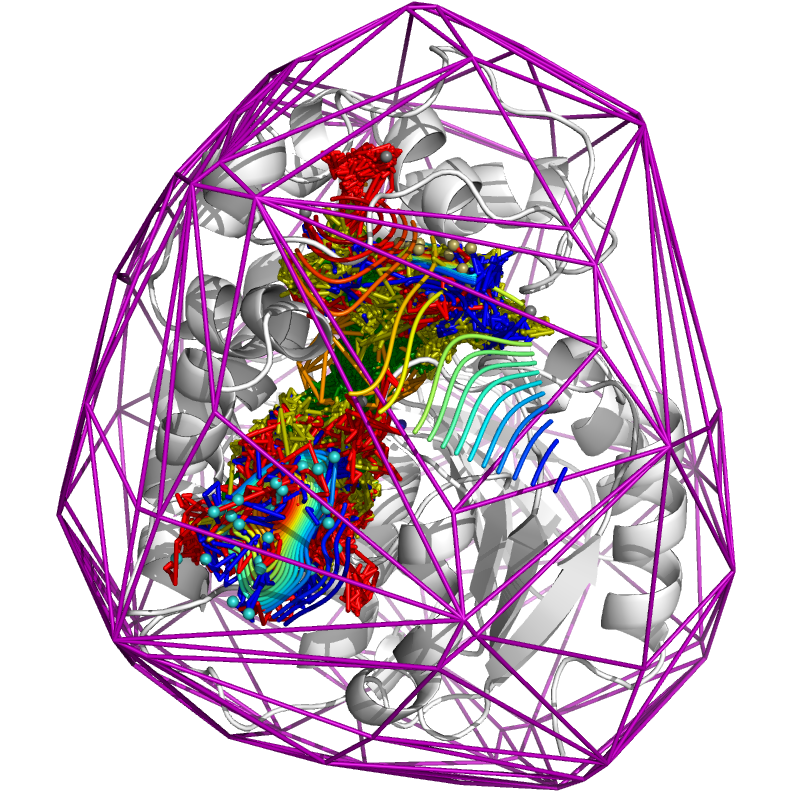
\includegraphics[width=0.5\textwidth]{Tut6.1.png}
\caption{Results of AQUA-DUCT calculations and clustering using sample data \#3. The \textit{Scope} is shown as a purple shape, the \textit{Object} as an orange shape, paths are shown as colour-coded lines, clusters are shown as coloured spheres, and cluster areas as coloured isolines.}
\label{Tut6.1}
\end{figure}

Using this command, the user will obtain information about all objects for which the options were set to \texttt{True} in the configuration file in the \texttt{[visualize]} section. As the user may notice, objects in the PyMOL session are both split according to the particular types of the traced molecules, as well as standard visualization linking the types of molecules being traced, is provided. The obtained clusters are relatively small in number of inlets, however, it can be seen that they consist of both \textbf{WAT} and \textbf{ACN} molecules. For further analysis, the user does not need to visualize all possible objects and types of paths generated by AQUA-DUCT. Moreover, there is a possibility to change the colours of clusters in such a way as to distinguish the inlets belonging to different types of molecules being traced. To simplify the visualization, change the clusters' colours and save the PyMOL session, the user should type in the command line:
\begin{lstlisting}
python 6_visualize_results.py --keep 'molecule cluster scope object raw' --discard 'master io all paths smooth' --force-color 'cluster_1 pink cluster_2 forest cluster_1_ACN hotpink cluster_2_ACN green cluster_1_WAT pink cluster_2_WAT forest' --save-session session.pse 
\end{lstlisting}
\begin{figure}[ht!]
\centering
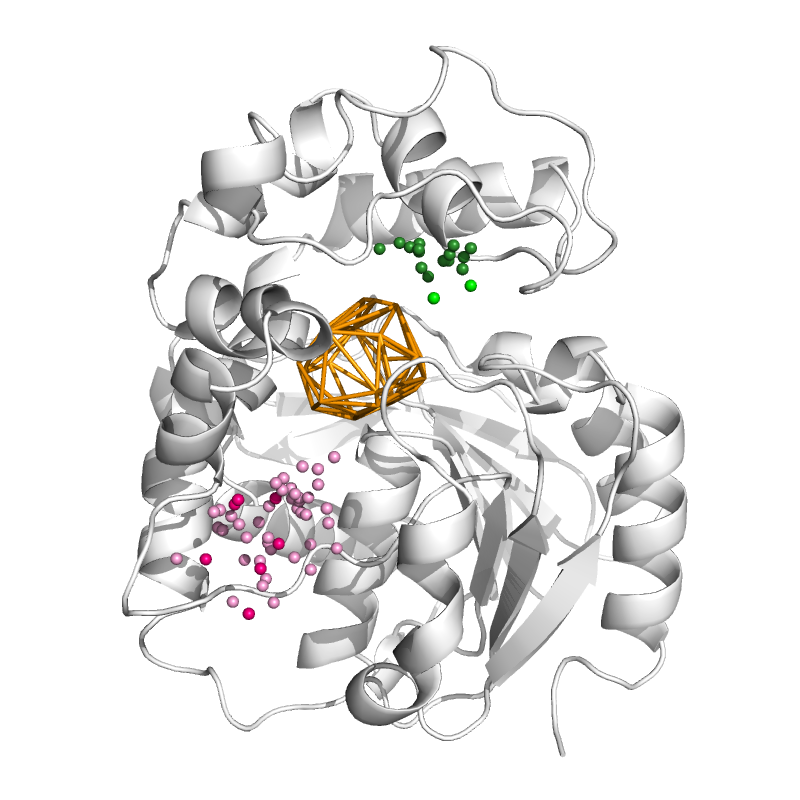
\includegraphics[width=0.5\textwidth]{Tut6.2.png}
\caption{Visualization of results in PyMOL. The following PyMOL objects are shown: \texttt{molecule0}, \texttt{object\_shape0}, \texttt{cluster\_1\_ACN} (hotpink), \texttt{cluster\_2\_ACN} (green), \texttt{cluster\_1\_WAT} (pink), \texttt{cluster\_2\_WAT} (forest).}
\label{Tut6.2}
\end{figure}

Since the main emphasis of this tutorial is on the analysis of hot-spots and pockets for particular solvent, therefore, it is necessary to run \emph{pond} analysis. With \emph{pond}, the user will perform the following calculations: pockets, local and global hot-spots for both solvents. First, calculations for acetonitrile molecules will be performed (on an Intel Core i7-4790 CPU @ 3.60 GHz machine they take approx. 1 minute). To do that, the user should type the following command in the command line:
\begin{lstlisting}
pond_run -c config.txt --debug-file pond_hs_ACN_local.log --pockets --hotspots --reference-calc --reference-mol 'resname ACN WAT' --paths-types 'ACN' --output-suffix 'local' -r Hotspots_local/ACN/ 
\end{lstlisting}
\emph{Pond} will calculate the local pockets and hot-spots for acetonitrile molecules. For multiple solvents analysis, it is important to remember about the proper use of options \texttt{-{}-reference-mol} and \texttt{-{}-paths-types}. The \texttt{-{}-reference-mol} option allows selecting for which type of molecules present in the system the reference density will be calculated. In the case of multiple solvent, all types of solvents present in the system should be taken into account for the calculations, therefore, in the above command, the user should include both \textbf{ACN} and \textbf{WAT} molecules. In turn, the \texttt{-{}-paths-types} option limits calculations to the given paths types. In the analysed case, the user wants to perform the calculations for acetonitrile molecules, that is why the argument used with this option is set to 'ACN'. Using the \texttt{-{}-output-suffix} option is beneficial because adding an appropriate suffix to the output files can help the user identify the type of data for which the calculations were performed. 
The user can find some useful information, both in the command line as well as in the created output file, e.g., \texttt{Reference number of molecules} in [molecules], \texttt{Reference density} in [molecules/Å\( \displaystyle ^{3}\)] and \texttt{Reference value} in [kJ/mol/K]. In the command line, the user should see the following information for the performed calculations: 
\begin{lstlisting}[columns=fullflexible]
Reference number of molecules: 3411 [molecules].
Reference density: 0.0509 [molecules/A^3].
Reference value: 7.4281 [kJ/mol/K].
\end{lstlisting}
Once the local pockets and hot-spots are calculated, it is time to calculate the same features with \texttt{-{}-raw} option to get a global information. This time, there is no need to recalculate the reference density value, since this has been already done. The user can enter the reference value that has just been calculated. The below calculations take approx. 20 seconds on an Intel Core i7-4790 CPU @ 3.60 GHz machine. In this situation, the user should write in the command line:
\begin{lstlisting}
pond_run -c config.txt --debug-file pond_hs_ACN_global.log --pockets --hotspots --reference-value 7.4281 --paths-types 'ACN' --raw --output-suffix 'global' -r Hotspots_global/ACN/ 
\end{lstlisting}
The user can now perform the corresponding calculations for water molecules. The command will be almost identical, but the user should remember to change the argument of the \texttt{-{}-paths-types} option. The below calculations take approx. 30 seconds on an Intel Core i7-4790 CPU @ 3.60 GHz machine. For local pockets and hot-spots the user should write in the command line:
\begin{lstlisting}
pond_run -c config.txt --debug-file pond_hs_WAT_local.log --pockets --hotspots --reference-value 7.4281 --paths-types 'WAT' --output-suffix 'local' -r Hotspots_local/WAT/ 
\end{lstlisting}
For global pockets and hot-spots, the user should write in the command line (on an Intel Core i7-4790 CPU @ 3.60 GHz machine the calculations take approx. 2 minutes):
\begin{lstlisting}
pond_run -c config.txt --debug-file pond_hs_WAT_global.log --pockets --hotspots --reference-value 7.4281 --paths-types 'WAT' --output-suffix 'global' --raw -r Hotspots_global/WAT/ 
\end{lstlisting}
When all pockets and hot-spots are calculated, the user can load the results into the previously saved session. As explained in the Tutorial 4, the user can change size of the hot-spots using the \texttt{hs\_resize.py} script from the AQUA-DUCT package. In the PyMOL console, the user should type:
\begin{lstlisting}[columns=fullflexible]
run /path/to/hs_resize.py
hs_resize /path/to/pond_meta_ACN_local.json, hotspots_full_ACN_local
hs_resize /path/to/pond_meta_WAT_local.json, hotspots_full_WAT_local
hs_resize /path/to/pond_meta_ACN_global.json, hotspots_full_ACN_global
hs_resize /path/to/pond_meta_WAT_global.json, hotspots_full_WAT_global
\end{lstlisting}
where \texttt{path/to/hs\_resize.py} should be replaced by the exact path to the script and \texttt{path/to/pond\_meta\_ACN\_local.json}, \texttt{path/to/pond\_meta\_WAT\_local.json},\newline \texttt{path/to/pond\_meta\_ACN\_global.json}, and \newline \texttt{path/to/pond\_meta\_WAT\_global.json} by the exact path to the \texttt{.json} file.
In addition to changing the hot-spots size, the user may also change their colours in the \texttt{color} settings in PyMOL, e.g. the user can set \texttt{hotspots\_full\_ACN\_local} to brightorange, \texttt{hotspots\_full\_WAT\_local} to lightblue, \texttt{hotspots\_full\_ACN\_global} \hfill to \hfill orange \hfill and \newline \texttt{hotspots\_full\_WAT\_global} to blue (Figure \ref{Tut6.3} and Figure \ref{Tut6.4}).

\begin{figure}[ht!]
\centering
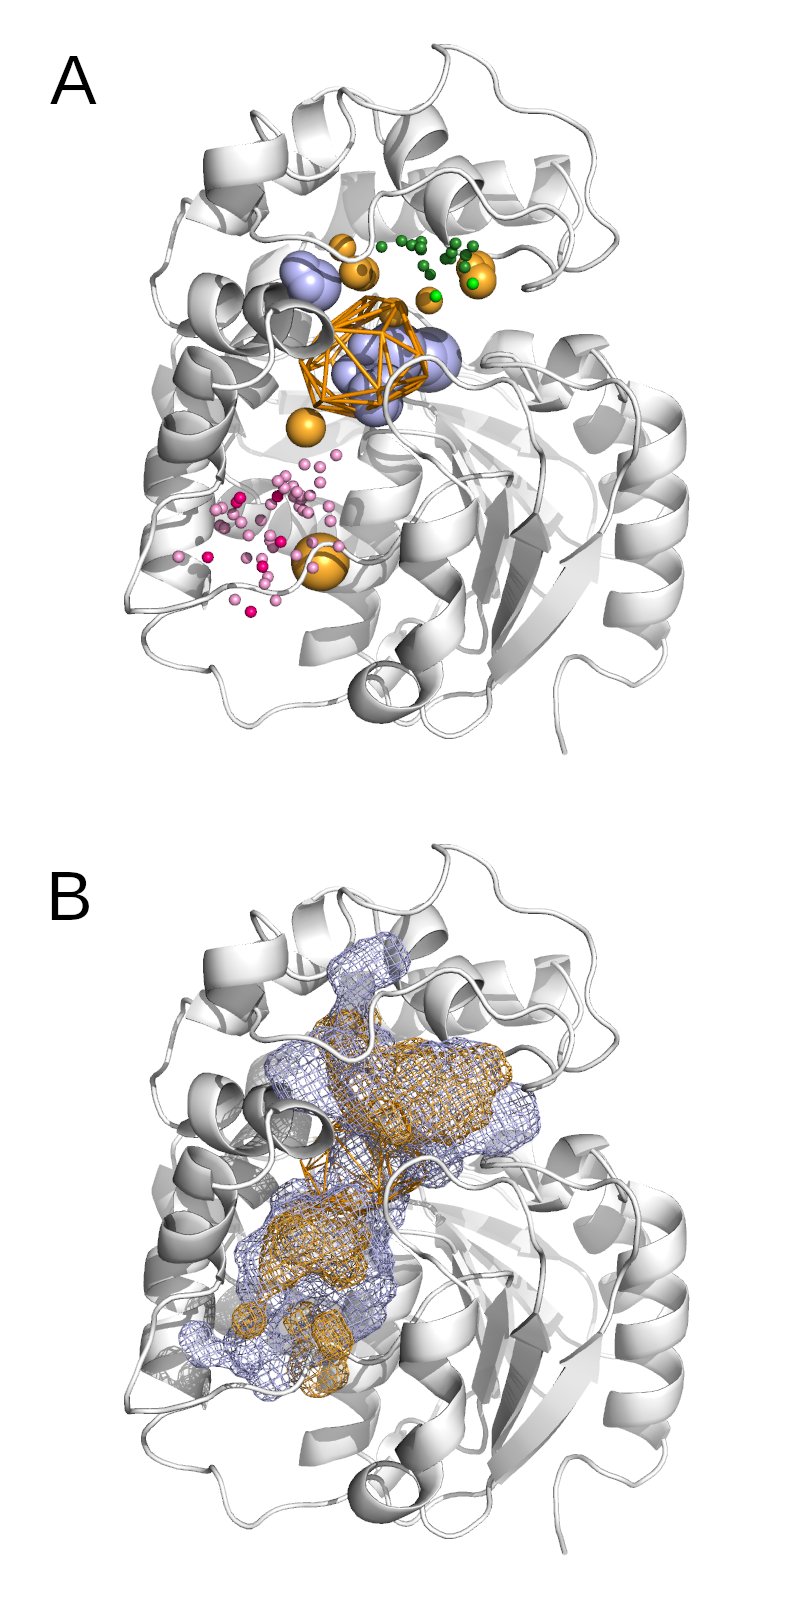
\includegraphics[width=0.5\textwidth]{Tut6.3.png}
\caption{Visualization of results in PyMOL: A) clusters and local hot-spots, B) inner pockets for acetonitrile and water molecules. The following PyMOL objects are shown: \texttt{molecule0}, \texttt{object\_shape0}, \texttt{cluster\_1\_ACN} (hotpink), \texttt{cluster\_2\_ACN} (green), \texttt{cluster\_1\_WAT} (pink), \texttt{cluster\_2\_WAT} (forest), \texttt{hotspots\_full\_ACN\_local} (brightorange spheres), \texttt{hotspots\_full\_WAT\_local} (lightblue spheres), \texttt{inner\_full\_ACN\_local} (brightorange mesh), \texttt{inner\_full\_WAT\_local} (lightblue spheres). The size of the hot-spots reflects their local density.}
\label{Tut6.3}
\end{figure}

\begin{figure}[ht!]
\centering
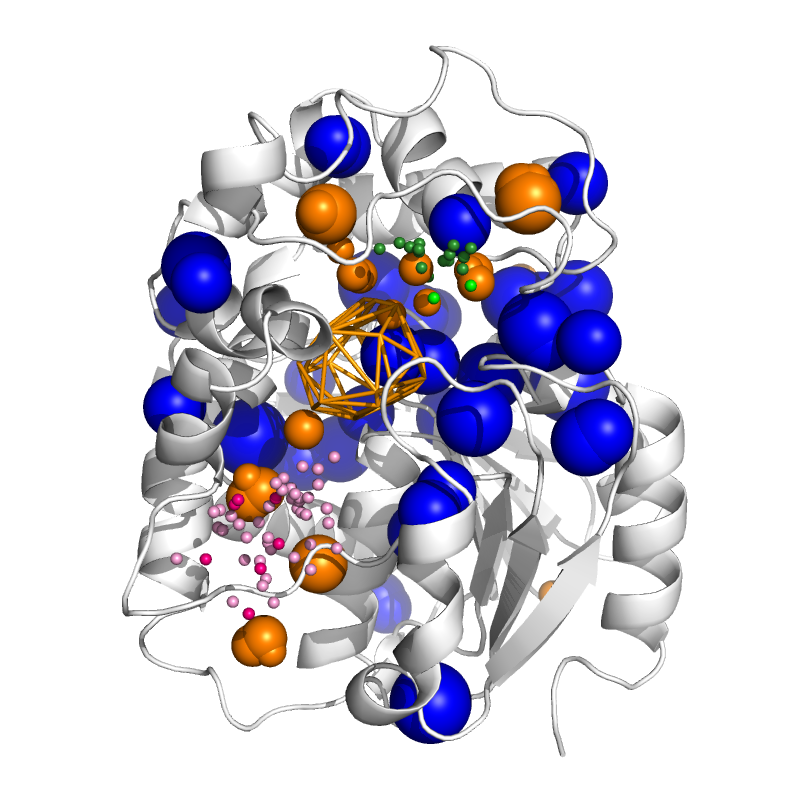
\includegraphics[width=0.5\textwidth]{Tut6.4.png}
\caption{Visualization of results in PyMOL: clusters and global hot-spots. The following PyMOL objects are shown: \texttt{molecule0}, \texttt{object\_shape0}, \texttt{cluster\_1\_ACN} (hotpink), \texttt{cluster\_2\_ACN} (green), \texttt{cluster\_1\_WAT} (pink), \texttt{cluster\_2\_WAT} (forest), \texttt{hotspots\_full\_ACN\_global} (orange), \texttt{hotspots\_full\_WAT\_global} (blue). The size of the hot-spots reflects their local density.}
\label{Tut6.4}
\end{figure}

The user can now determine in which regions hot-spots are most likely to be found, and thus, analyse these places more precisely, e.g. in the context of possible protein engineering or drug design. As the user may see, in the case of local hot-spots, for water molecules, they are placed within the close vicinity of the active site indicated by the \texttt{Object}, while for acetonitrile molecules, they occupy more distant regions.
In Figure \ref{Tut6.3} B, the user can see the differences in the inner pockets for acetonitrile and water molecules. The volume of acetonitrile's inner pocket is smaller, since the proportion of the acetonitrile molecules in the system was much smaller compared to water molecules and the acetonitrile molecules penetrate the protein's interior to a lesser extent. The volumes of inner (also outer) pockets can be found in the \texttt{volumes\_ACN\_local.dat} and \texttt{volumes\_WAT\_local.dat} files which were saved in the respective directories during the \emph{pond} calculations. Herein, the inner pocket volume for acetonitrile molecules is 260 Å\( \displaystyle ^{3}\), while for water molecules the inner pocket volume is almost twice as large and amounts to 477 Å\( \displaystyle ^{3}\).

Typically, in the case of the multiple solvent analysis, calculations are performed for at least few different solvents. Usually, several different combinations are analysed (e.g. water+acetamide, water+benzene, water+isopropanol, water+methanol, water+acetonitrile, etc.), in which the vast majority are water molecules, while the cosolvent makes up a certain percentage of the system. The authors suggest that in such cases, the analysis should be as follows: conduct pockets and hot-spots analysis for a system containing water molecules as pure solvent (considered as a reference system, as data set \#2), conduct pockets and hot-spots analysis for mixed systems while limiting the type of molecules present in the system only to the cosolvent molecules (e.g. acetonitrile). Results obtained from different (co)solvents can then be superimposed in PyMOL on one structure and the user may identify regions in the macromolecule which overlap in terms of presence of different types of hot-spots as well as determine those which are unique.     

\section{Author Contributions}
%%%%%%%%%%%%%%%%
% This section must describe the actual contributions of
% author. Since this is an electronic-only journal, there is
% no length limit when you describe the authors' contributions,
% so we recommend describing what they actually did rather than
% simply categorizing them in a small number of
% predefined roles as might be done in other journals.
%
% See the policies ``Policies on Authorship'' section of https://livecoms.github.io
% for more information on deciding on authorship and author order.
%%%%%%%%%%%%%%%%

KM and AR conceived of and wrote all the online tutorials and the User Guide, KM and MB prepared the sample data sets, PW maintains the \githubrepository, and KM, AR, PW, MB, and AG wrote this article.

% We suggest you preserve this comment:
For a more detailed description of author contributions,
see the GitHub issue tracking and changelog at \githubrepository.

\section{Other Contributions}
%%%%%%%%%%%%%%%
% You should include all people who have filed issues that were
% accepted into the paper, or that upon discussion altered what was in the paper.
% Multiple significant contributions might mean that the contributor
% should be moved to authorship at the discretion of the a
%
% See the policies ``Policies on Authorship'' section of https://livecoms.github.io for
% more information on deciding on authorship and author order.
%%%%%%%%%%%%%%%

The authors would like to acknowledge Tomasz Magdziarz and Michał Banas for their contribution in AQUA-DUCT development. The authors thank Weronika Bagrowska for the final inspection and verification of the presented tutorials.

% We suggest you preserve this comment:
For a more detailed description of contributions from the community and others, see the GitHub issue tracking and changelog at \githubrepository.

\section{Potentially Conflicting Interests}
%%%%%%%
%Declare any potentially competing interests, financial or otherwise
%%%%%%%

The authors declare no potential conflict of interests.
%Declare any potentially conflicting interests here, whether or not they pose an actual conflict in your view.

\section{Funding Information}
%%%%%%%
% Authors should acknowledge funding sources here. Reference specific grants.
%%%%%%%
This work was supported by the National Science Centre, Poland [DEC-2013/10/E/NZ1/00649 and \newline DEC-2015/18/M/NZ1/00427]. \newline
The work of Maria Bzówka was supported by the Ministry of Science and Higher Education, Poland from the budget for science for the years 2019-2023, as a research project under the "Diamond Grant" programme [0141/DIA/2019/48].

\section*{Author Information}
\makeorcid

\bibliography{references}

%%%%%%%%%%%%%%%%%%%%%%%%%%%%%%%%%%%%%%%%%%%%%%%%%%%%%%%%%%%%
%%% APPENDICES
%%%%%%%%%%%%%%%%%%%%%%%%%%%%%%%%%%%%%%%%%%%%%%%%%%%%%%%%%%%%

%\appendix


\end{document}
